%\documentclass[12pt]{article}


\documentclass[12pt]{article}
\usepackage[backend=bibtex,natbib,style=numeric-comp,sorting=none, doi=false, isbn=false,url=false]{biblatex}
\usepackage{slashed}
\addbibresource{refs}
\input epsf.sty

\pdfoutput=1

% Use Chancery Font
\DeclareFontFamily{OT1}{pzc}{}
\DeclareFontShape{OT1}{pzc}{m}{it}{<-> s * [1.10] pzcmi7t}{}
\DeclareMathAlphabet{\mathpzc}{OT1}{pzc}{m}{it}
\newcommand{\josh}[1]{\textcolor{blue}{[Joshua: #1]}}
\newcommand{\cw}[1]{\textcolor{gray}{[Charles: #1]}}
%\usepackage{chngcntr}
%\counterwithout{equation}{section}



\newcommand{\bb}[1]{\mathbb{#1}}
\newcommand{\wt}[1]{\widetilde{#1}}
\newcommand{\ol}[1]{\overline{#1}}
\newcommand{\mc}[1]{\mathcal{#1}}
\newcommand{\Sym}{\mathrm{Sym}}
\newcommand{\hmch}{\hat{\mc{H}}}
\newcommand{\citeme}[1][]{{\color{red}[*#1]}}

\usepackage{stmaryrd}


\usepackage{draft}
\usepackage[weather]{ifsym}

\usepackage{hyperref}
\usepackage{graphicx,color,subfig}
\usepackage{skak}
\usepackage{empheq}
\usepackage{tikz}
\usepackage{bbm}

% Use Chancery Font
\DeclareFontFamily{OT1}{pzc}{}
\DeclareFontShape{OT1}{pzc}{m}{it}{<-> s * [1.10] pzcmi7t}{}
\DeclareMathAlphabet{\mathpzc}{OT1}{pzc}{m}{it}

\usetikzlibrary{calc}
\usetikzlibrary{snakes}
\usetikzlibrary{arrows.meta}
\usetikzlibrary{decorations.pathmorphing}
\usetikzlibrary{decorations.markings}
\usetikzlibrary{bending}
\tikzset{snake it/.style={decorate, decoration=snake}}
\usetikzlibrary{shapes.misc}
\tikzset{cross/.style={cross out, draw=black, minimum size=2*(#1-\pgflinewidth), inner sep=0pt, outer sep=0pt},
%default radius will be 1pt.
cross/.default={1pt}}

\usepackage[T1]{fontenc}
\usepackage{esint}
\usepackage{lmodern}

\newcommand{\fixme}[1]{{\bf {\color{red}[#1]}}}
\newcommand{\vv}[1]{\left\langle #1 \right\rangle}
\newcommand{\un}[1]{\underline{#1}}
\newcommand{\BL}[1]{{ {\color{blue}[#1]}}}

\newcommand{\bgcom}[1]{\fixme{BG: #1}}

\def\be#1\ee{\begin{align}#1\end{align}}
\newcommand\nn{\nonumber}

\newcommand{\calA}{\mathcal{A}}
\newcommand{\bz}{\bar{z}}


\definecolor{dark green}{rgb}{0.7,1,0.64}

\usepackage{listings}
\usepackage{xcolor}

\definecolor{codegreen}{rgb}{0,0.6,0}
\definecolor{codegray}{rgb}{0.5,0.5,0.5}
\definecolor{codepurple}{rgb}{0.58,0,0.82}
\definecolor{backcolour}{rgb}{0.95,0.95,0.92}

\lstdefinestyle{myStyle}{
    belowcaptionskip=1\baselineskip,
    breaklines=true,
    frame=none,
    numbers=none,
    basicstyle=\footnotesize\ttfamily,
    keywordstyle=\bfseries\color{green!40!black},
    commentstyle=\itshape\color{purple!40!black},
    identifierstyle=\color{blue},
    backgroundcolor=\color{gray!10!white},
    tabsize=2,
}



\lstset{style=myStyle}
\usepackage{array}
\usepackage{physics}

\begin{document}

\unitlength = .8mm


\section{The holographic duality}
We begin by reviewing the holographic duality, on top of which the MST conjecture is built. Start from the decoupling limit of the extremal black 1-brane solution of type IIB string theory, described in terms of the string frame metric, the dilaton $\Phi$, and the RR 2-form potential $C_2$ as
\ie\label{dsaiibdoness}
& ds_{\rm str}^2 = (\wt f_1(r))^{-{1\over 2}} (-dt^2 + dx^2) + (\wt f_1(r))^{1\over 2} (dr^2 + r^2 d\Omega_7^2),
\\
& e^\Phi = (\wt f_1(r))^{1\over 2},~~~~ C_2 =  \wt f_1^{-1} dt \wedge dx,
\\
& \wt f_1(r) = {c_1 N\over r^6},~~~~ c_1 = 32 \pi^2 g_B \ell_B^6 = 32\pi^2 g_B^{-{1\over 2}}M_{\rm pl}^{-6},
\fe
where $\ell_B$ is the type IIB string length, and $g_B$ is the type IIB string coupling (defined as the ratio between the F1 and D1 string tensions in the absence of RR axion and dilaton expectation value).
The standard holographic dictionary suggests an exact dual description in terms of the 2D ${\cal N}=(8,8)$ $U(N)$ SYM characterized by the gauge field $A_\mu$, adjoint scalar fields $\phi^i$, and adjoint fermions $\lambda_{\A +}$, $\lambda_{\da -}$. Here $i=1,\cdots,8$ is a vector index with respect to the $so(8)_R$ symmetry, and $\A, \da$ are chiral and anti-chiral spinor indices with respect to the $so(8)_R$. The Lorentzian action reads
\ie
S & = {1\over g_{\rm YM}^2} \int d^2x\, {\rm tr} \bigg( - {1\over 4} F_{\mu\nu} F^{\mu\nu} - {1\over 2} D_\mu \phi^i D^\mu \phi^i + {1\over 4} [\phi^i, \phi^j]^2
\\
&~~~~~~~~~~~~~~~~~~~ -  \lambda_{\A+} D_- \lambda_{\A+} -  \lambda_{\da -} D_+ \lambda_{\da-} - \lambda_{\A+}\C^i_{\A\da} [\phi^i, \lambda_{\da-} ] \bigg),
\fe
where the gauge coupling $g_{\rm YM}$ is identified as
\ie\label{gymdict}
g_{\rm YM}^2 = { g_B\over 2\pi \ell_B^2}
\fe
and $D_\mu \equiv\partial_\mu - i [A_\mu, \cdot]$ in the adjoint, with the trace taken in the fundamental.
Applying the S-duality transformation to (\ref{dsaiibdoness}) yields the purely (NS,NS) spacetime background\footnote{Note that the 3-form field strength $H_3 = dB_2 = e^{2\Phi} {6dr\over r}\wedge dt\wedge dx$ obeys $\wt g_B^{-2}\int_{S^7} e^{-2\Phi} * H = (2\pi \sqrt{\A'})^6 N$, which is the electric (NS,NS) flux sourced by $N$ fundamental strings.}
\ie\label{f1sdualbg}
& d s_{\rm str}^2 =  (\wt f_1(r))^{-1} (-dt^2 + dx^2) + dr^2 + r^2 d\Omega_7^2,
\\
& e^{\Phi} = (\wt f_1(r))^{-{1\over 2}},~~~~ B_2 = \wt f_1^{-1} dt\wedge dx,
\\
& \wt f_1(r) = {c_1 N\over r^6},~~~~ c_1 = 32\pi^2 \wt g_B^{1\over 2} M_{\rm pl}^{-6} = 32\pi^2 \wt g_B^2 \wt\ell_B^6,
\fe
where $\wt g_B = g_B^{-1}$ and $\wt\ell_B = g_B^{1\over 2} \ell_B$ are the string coupling and length in the dual frame.
It is important to keep the order of limits explicit. The geometries (\ref{dsaiibdoness}) and (\ref{f1sdualbg}) are already post-decoupling near-horizon backgrounds. The NCOS/SYM map used below is instead derived from the parent asymptotically flat D1-F1 system (a D1-brane with $N$ units of electric flux), with the decoupling limit taken there; only after that derivation do we embed the result into the holographic channel represented by (\ref{dsaiibdoness}), (\ref{f1sdualbg}) \cite{seiberg2000stringsbackgroundelectricfield,klebanov200011dimensionalncosun,yin2026foundationsofstringtheory}.

\subsection{NCOS in the S-dual frame}
To derive the NCOS/SYM dictionary, we start from the parent flat-space D1 system carrying $N$ electric-flux quanta (equivalently a D1-F1 bound state), and take its NCOS decoupling limit \cite{seiberg2000stringsbackgroundelectricfield,klebanov200011dimensionalncosun}. We first describe the intrinsic worldsheet BCFT data of this D1-brane in a constant electric background, and only afterwards match to the holographic variables.
\subsubsection{Definition of NCOS}
In the S-dual frame, define
\ie\label{edefsingleflux}
\widetilde E \equiv 2\pi \wt\ell_B^2 F_{01}.
\fe
Denote
\ie\label{ncosbdef}
{\cal B}_{\alpha\beta}\equiv B_{\alpha\beta}+2\pi\wt\ell_B^2 F_{\alpha\beta}.
\fe
Using the D-brane effective action with $G+B+2\pi\A'F$ \cite{yin2026foundationsofstringtheory} (chapter 14 equations (14.53), (14.79)), the boundary condition is
\ie\label{ncosbcftbdry}
\eta_{\alpha\beta}\partial_n X^\beta + {\cal B}_{\alpha\beta}\partial_t X^\beta\Big|_{\partial\Sigma}=0,~~~~\alpha,\beta=0,1.
\fe
This is the standard mixed Neumann condition for open strings in constant background field \cite{seiberg1999stringtheorynoncommutativegeometry} (equation (2.2)). The Seiberg-Witten open-string data are
\ie\label{ncosswdata}
G^{\alpha\beta}=\left({1\over \eta+{\cal B}}\right)^{\alpha\beta}_{\!S},~~~~
\theta^{\alpha\beta}=2\pi\wt\ell_B^2\left({1\over \eta+{\cal B}}\right)^{\alpha\beta}_{\!A},
\fe
and for a purely electric field ($B_{01}=0$, so ${\cal B}_{01}=\widetilde E$) in 1+1 dimensions, matching equation (2.5) of \cite{seiberg1999stringtheorynoncommutativegeometry},
\ie\label{ncos1plus1}
G_{00}=-(1-\widetilde E^2),~~~~G_{11}=1-\widetilde E^2,~~~~
\theta^{01}={2\pi\wt\ell_B^2 \widetilde E\over 1-\widetilde E^2}.
\fe
The open-string coupling (denoted $G_0$ in \cite{klebanov200011dimensionalncosun}, equation (2) for $M=1$ and equation (3) for general $M$) follows from \cite{seiberg1999stringtheorynoncommutativegeometry} (equation (2.44)):
\ie\label{gzerodef}
G_o^2=\wt g_B\sqrt{{\det G\over \det(\eta+{\cal B})}}.
\fe
Conceptually, this relation is obtained by rewriting the same disk-level D-brane physics in two equivalent parameterizations: the ``closed-string'' variables $(\eta,{\cal B},\wt g_B)$ and the ``open-string'' variables $(G,\theta,G_o)$. Matching the normalization of the DBI action (equivalently the disk partition function) in the two descriptions fixes the Jacobian factor $\sqrt{\det G/\det(\eta+{\cal B})}$, which is why (\ref{gzerodef}) and the equation above are kinematic redefinitions rather than an additional dynamical input.
For $B_{01}=0$, one gets explicitly
\ie
G_o^2=\wt g_B\sqrt{1-\widetilde E^2}.
\fe
The effective NCOS string scale is defined by the effective open-string tension (equivalently the open-string mass-shell relation with metric (\ref{ncos1plus1})) as
\ie\label{alphaeffdef}
\A'_{\rm eff}\equiv {\wt\ell_B^2\over 1-\widetilde E^2},
\fe
so that
\ie
{1\over 2\pi\A'_{\rm eff}}={1-\widetilde E^2\over 2\pi\wt\ell_B^2}.
\fe
This denominator is the near-critical electric-field suppression of the net string tension along the electric direction: the electric force on the charged endpoints partially cancels the bare tension, leaving the effective tension above \cite{seiberg2000stringsbackgroundelectricfield}. Equivalently, in open-string variables the metric (\ref{ncos1plus1}) rescales the longitudinal mass-shell relation by $1-\widetilde E^2$, and rewriting in canonical units gives the same $\A'_{\rm eff}$. This is the standard NCOS definition (cf.\ equation (2.7) of \cite{seiberg2000stringsbackgroundelectricfield}).
A useful way to see why the dependence is exactly $1-\widetilde E^2$ (rather than, say, $1-\widetilde E$) is that the same invariant combination controls all electric-field effects in the D1 Born-Infeld system: the action density, electric displacement, and criticality bound all involve $\sqrt{1-\widetilde E^2}$. Therefore the longitudinal open-string tension must vanish quadratically as $\widetilde E\to 1$, giving $T_{\rm eff}=T_{\rm F1}(1-\widetilde E^2)$ with $T_{\rm F1}=1/(2\pi\wt\ell_B^2)$.
From the worldsheet side, the same factor is encoded in the open-string metric (\ref{ncos1plus1}). Since the open-string Hamiltonian uses $G^{\alpha\beta}p_\alpha p_\beta$, canonical normalization of the longitudinal coordinates absorbs the factor $1-\widetilde E^2$ into the inverse slope, so the spectrum is naturally written with $\A'_{\rm eff}=\wt\ell_B^2/(1-\widetilde E^2)$. This is why the NCOS limit keeps $\A'_{\rm eff}$ fixed while sending $\wt\ell_B^2\to 0$ and $\widetilde E\to 1$: the bare closed-string scale is removed, but the finite effective open-string scale is retained.
In intrinsic BCFT variables, one often parameterizes the NCOS scaling as
\ie\label{ncoslimit}
\widetilde E\to 1,~~~~\A'_{\rm eff}~{\rm fixed},~~~~G_0~{\rm fixed}.
\fe
This scaling retains the interacting open-string sector at finite scale while removing the bare closed-string scale.
\subsubsection{Boundary OPE and Moyal phases}
\noindent
At the level of boundary CFT, the symmetric and antisymmetric tensors in (\ref{ncosswdata}) enter differently. The boundary two-point function takes the standard form
\ie
\langle X^\alpha(\tau)X^\beta(0)\rangle
=-2\wt\ell_B^2 G^{\alpha\beta}\ln|\tau|
 + {i\over 2}\theta^{\alpha\beta}\,\epsilon(\tau),
\fe
where $\epsilon(\tau)\equiv \mathrm{sgn}(\tau)$. Plugging (\ref{ncos1plus1}) into this gives
\ie
\langle X^0(\tau)X^0(0)\rangle=2\A'_{\rm eff}\ln|\tau|,\qquad
\langle X^1(\tau)X^1(0)\rangle=-2\A'_{\rm eff}\ln|\tau|,
\fe
\ie
\langle X^0(\tau)X^1(0)\rangle=+{i\over 2}\theta^{01}\epsilon(\tau),\qquad
\langle X^1(\tau)X^0(0)\rangle=-{i\over 2}\theta^{01}\epsilon(\tau),
\qquad
\theta^{01}=2\pi\A'_{\rm eff}\widetilde E.
\fe
In lightcone coordinates $X^\pm\equiv X^0\pm X^1$, one has
\ie
G^{++}=G^{--}=0,\qquad G^{+-}=G^{-+}=-{2\over 1-\widetilde E^2},\qquad
\theta^{++}=\theta^{--}=0,\qquad \theta^{+-}=-\theta^{-+}=-2\theta^{01},
\fe
and therefore
\ie
\langle X^+(\tau)X^-(0)\rangle
= 4\A'_{\rm eff}\ln|\tau|
- i\,\theta^{01}\epsilon(\tau),
\qquad
\langle X^-(\tau)X^+(0)\rangle
= 4\A'_{\rm eff}\ln|\tau|
+ i\,\theta^{01}\epsilon(\tau),
\fe
with $\langle X^\pm(\tau)X^\pm(0)\rangle=0$ at this level. This makes explicit that the logarithmic part is controlled by the open metric ($G$), while the ordering-dependent phase is controlled by $\theta$.
For transverse coordinates $X^i$ ($i=2,\dots,9$), the electric background does not induce a noncommutative phase: $\theta^{i\alpha}=\theta^{ij}=0$. Their two-point function keeps the usual logarithmic form set by the transverse open metric ($G_{ij}=\delta_{ij}$ in this setup), so in these conventions
\ie
\langle X^i(\tau)X^j(0)\rangle\sim -2\wt\ell_B^2\delta^{ij}\ln|\tau|,
\fe
with no $\epsilon(\tau)$ term. A form with $\A'_{\rm eff}$ in the transverse correlator is obtained only after an additional transverse coordinate rescaling.
Therefore $G^{\alpha\beta}$ controls the logarithmic term and therefore the scaling dimensions and mass shell (equivalently the open-string Hamiltonian) through $G^{\alpha\beta}k_\alpha k_\beta$, while $\theta^{\alpha\beta}$ controls the discontinuous phase. Restricting to no transverse momenta ($k_i=q_i=0$) and using lightcone variables $k_\pm\equiv k_0\pm k_1$, $q_\pm\equiv q_0\pm q_1$, with
\ie
V_k(\tau)\equiv \exp\!\left[{i\over 2}\left(k_+X^-+k_-X^+\right)\right],
\fe
the boundary OPE can be written as
\ie
V_k(\tau)V_q(0)\sim
|\tau|^{-\A'_{\rm eff}(k_+q_-+k_-q_+)}
\exp\!\left[-{i\over 4}\theta^{01}(k_-q_+-k_+q_-)\epsilon(\tau)\right]
V_{k+q}(0).
\fe
Thus $\theta$ changes correlation functions and amplitudes by Moyal-type momentum phases, whereas $G$ sets the kinematic spectrum. In the present 1+1 electric case, $\theta^{01}=2\pi\A'_{\rm eff}\widetilde E\to 2\pi\A'_{\rm eff}$ as $\widetilde E\to 1$, yielding finite spacetime noncommutativity at fixed open-string scale \cite{seiberg1999stringtheorynoncommutativegeometry,seiberg2000stringsbackgroundelectricfield,gopakumar2000sdualitynoncommutativegaugetheory}. Therefore one keeps a finite interacting open-string sector with spacetime noncommutativity; see especially equations (4.1), (4.2), (4.3), (4.6), (4.7) of \cite{seiberg2000stringsbackgroundelectricfield} and equation (3.4) of \cite{gopakumar2000sdualitynoncommutativegaugetheory}.
\subsubsection{Bulk operators in the critical-field limit}
\noindent
The boundary OPE above is the restriction of the exact upper-half-plane propagator for a D-brane in constant background field \cite{seiberg1999stringtheorynoncommutativegeometry}. For longitudinal indices $\alpha,\beta=0,1$, and suppressing additive constants, it can be written in our conventions as
\ie\label{ncosbulkuhp}
\langle X^\alpha(z,\bar z)X^\beta(w,\bar w)\rangle
=-\wt\ell_B^2\left[
\eta^{\alpha\beta}\ln|z-w|
-\eta^{\alpha\beta}\ln|z-\bar w|
+G^{\alpha\beta}\ln|z-\bar w|^2
+{1\over 2\pi\wt\ell_B^2}\theta^{\alpha\beta}
\ln\!\frac{z-\bar w}{\bar z-w}
\right],
\fe
with the branch of the last logarithm chosen so that its cut lies below the upper half plane. Restricting $z,w$ to the boundary from ${\rm Im}\,z,{\rm Im}\,w>0$ then reproduces the boundary correlator used above. The first term is the direct bulk contraction controlled by the closed metric $\eta$, while the image terms are governed by the open data $(G,\theta)$.

For the present electric D1 system it is convenient to again use $X^\pm=X^0\pm X^1$. Plugging (\ref{ncos1plus1}) into (\ref{ncosbulkuhp}) gives
\ie\label{ncosbulklightcone}
\langle X^+(z,\bar z)X^-(w,\bar w)\rangle
=2\wt\ell_B^2\ln\!\left|{z-w\over z-\bar w}\right|
+2\A'_{\rm eff}\ln|z-\bar w|^2
+{\theta^{01}\over \pi}\ln\!\frac{z-\bar w}{\bar z-w},
\fe
\ie
\langle X^-(z,\bar z)X^+(w,\bar w)\rangle
=2\wt\ell_B^2\ln\!\left|{z-w\over z-\bar w}\right|
+2\A'_{\rm eff}\ln|z-\bar w|^2
-{\theta^{01}\over \pi}\ln\!\frac{z-\bar w}{\bar z-w},
\qquad
\langle X^\pm(z,\bar z)X^\pm(w,\bar w)\rangle=0.
\fe
The critical-field limit reorganizes these terms sharply. The direct interior contraction proportional to $\wt\ell_B^2$ vanishes, while $\theta^{01}\to 2\pi\A'_{\rm eff}$ and the image logarithm proportional to $\A'_{\rm eff}$ survives. Therefore
\ie\label{ncosbulkcritprop}
\langle X^+(z,\bar z)X^-(w,\bar w)\rangle_{\rm NCOS}
=4\A'_{\rm eff}\ln(z-\bar w),\qquad
\langle X^-(z,\bar z)X^+(w,\bar w)\rangle_{\rm NCOS}
=4\A'_{\rm eff}\ln(\bar z-w),
\fe
again with branch cuts chosen outside the disk (or, equivalently, below the upper half plane). Restricting these expressions back to the boundary reproduces the same holomorphic logarithm that appeared in the massless contour argument. This is the electric-field version of the Gomis-Ooguri/NRCS worldsheet reorganization, now expressed directly in the D1 electric variables of NCOS \cite{gomis2000nonrelativisticclosedstringtheory,seiberg2000stringsbackgroundelectricfield}.

The surviving bulk algebra is therefore entirely image-mediated. Using factorized normal ordering for the holomorphic and antiholomorphic pieces,
\ie\label{ncosbulkexp}
{\cal U}_{p,\bar p}(z,\bar z)\equiv
:\exp\!\left[{i\over 2}p_-X^+(z)\right]:
:\exp\!\left[{i\over 2}\bar p_+X^-(\bar z)\right]:,
\fe
the self-contraction inside one bulk insertion is
\ie
:\exp\!\left[{i\over 2}p_-X^+(z)\right]:
:\exp\!\left[{i\over 2}\bar p_+X^-(\bar z)\right]:
=(z-\bar z)^{-\A'_{\rm eff}p_-\bar p_+}
:\exp\!\left[{i\over 2}\left(p_-X^+(z)+\bar p_+X^-(\bar z)\right)\right]:.
\fe
For two such bulk insertions, only the crossed image contractions survive, so
\ie\label{ncosbulkbulk}
{\cal U}_{p,\bar p}(z,\bar z)\,
{\cal U}_{q,\bar q}(w,\bar w)
\sim
(z-\bar w)^{-\A'_{\rm eff}p_-\bar q_+}
(\bar z-w)^{-\A'_{\rm eff}\bar p_+q_-}
{\cal U}_{p+q,\bar p+\bar q}(w,\bar w).
\fe
Sending the bulk operator to the boundary, $z=\tau+iy$, $\bar z=\tau-iy$, yields
\ie\label{ncosbulkboundary}
{\cal U}_{p,\bar p}(\tau+iy,\tau-iy)
\sim
(2iy)^{-\A'_{\rm eff}p_-\bar p_+}
\exp\!\left[{i\over2}\left(\bar p_+X^-+p_-X^+\right)(\tau)\right],
\qquad y\to0^+,
\fe
namely the corresponding boundary vertex with $k_+=\bar p_+$ and $k_-=p_-$. Thus the critical limit produces a finite bulk-to-boundary algebra rather than a finite propagating unwound closed-string sector.

For transverse coordinates $X^i$, the electric field induces no noncommutative phase and no analogous $\A'_{\rm eff}$ enhancement. Their upper-half-plane propagators remain proportional to the bare closed-string scale $\wt\ell_B^2$, so in the strict NCOS limit no independent finite bulk algebra survives unless one simultaneously rescales transverse data. This is why the formulas above are written in the same $k_i=0$ longitudinal sector used throughout the present BCFT discussion.

This is the key difference from the Seiberg-Witten field-theory limit. There one sends $\wt\ell_B^2\to0$ at fixed $G$ and $\theta$, so the boundary propagator collapses to its discontinuous phase and the zero-slope/topological description becomes appropriate \cite{seiberg1999stringtheorynoncommutativegeometry}. In NCOS one instead keeps $\A'_{\rm eff}$ fixed, and the mixed logarithms (\ref{ncosbulkcritprop}) remain at the open-string scale. The result is not a pure star-product algebra for boundary operators, but a holomorphic bulk-boundary algebra that still knows about the finite NCOS string tension.

At the same time, this worldsheet limit does not resurrect a finite-energy non-compact closed-string spectrum. The scaling dimension of a genuine bulk closed-string vertex is still set by the direct $z-w$ contraction proportional to $\wt\ell_B^2\eta^{\alpha\beta}$, so keeping such a state on shell at fixed non-compact momentum requires energies of order $1/\wt\ell_B\to\infty$. Thus the algebra above only describes how longitudinal interior insertions collapse onto the boundary in the critical limit; the physical statement remains that unwound bulk closed strings decouple from finite-energy NCOS dynamics, in agreement with the threshold analysis below \cite{seiberg2000stringsbackgroundelectricfield,gopakumar2000sdualitynoncommutativegaugetheory}.
\subsubsection{Old derivation of nonrelativistic strings}
\noindent
The first-order longitudinal system used below was not introduced originally from the D1 boundary algebra. Historically, Seiberg, Susskind, and Toumbas emphasized that when the electric direction is compact, the same near-critical scaling that defines NCOS leaves a finite sector of wound closed strings \cite{seiberg2000stringsbackgroundelectricfield}. Gomis and Ooguri then isolated that closed-string sector and rewrote it as a first-order worldsheet theory, now usually called the Gomis-Ooguri or NRCS string \cite{gomis2000nonrelativisticclosedstringtheory}. Danielsson, Guijosa, and Kruczenski further recast the same limit as Wound String Theory, which makes the positive-winding sector manifest \cite{danielsson2000iiabwoundwrapped}. Since our later first-order formulas reuse the same longitudinal variables, it is useful to recall this older derivation explicitly.

It is important not to identify that flat Gomis-Ooguri parent background with the curved near-horizon F1 geometry (\ref{f1sdualbg}) used earlier in the holographic discussion. The relation is indirect. Before the near-horizon limit, the S-dual F1 solution is the asymptotically flat background
\ie\label{f1fullbg}
H_F(r)\equiv 1+\wt f_1(r)=1+{c_1N\over r^6},
\fe
\ie
ds_{\rm str}^2
=
H_F(r)^{-1}(-dt^2+dx^2)+dr^2+r^2d\Omega_7^2,
\qquad
e^\Phi = H_F(r)^{-{1\over 2}},
\fe
\ie
B_2=(1-H_F(r)^{-1})\,dt\wedge dx,
\fe
written in the same normalization conventions as (\ref{f1sdualbg}), with the asymptotic constant absorbed into the gauge choice for $B_2$. Dropping the asymptotic $1$ in $H_F$ gives the near-horizon metric (\ref{f1sdualbg}), while shifting $B_2$ by the constant two-form $dt\wedge dx$ puts the $B$-field in the gauge used there. Thus (\ref{f1sdualbg}) is the post-decoupling throat description, whereas the older NRCS derivation starts from the parent compact-background problem before that near-horizon step.

The bridge to the Gomis-Ooguri variables is therefore only local. Fix a radius $r=r_\ast$ and consider a worldsheet patch small compared with the radial variation scale of $H_F$. On that patch $H_F(r)$ may be treated as the constant number $H_\ast\equiv H_F(r_\ast)$. Introduce local coordinates
\ie\label{f1localcoords}
t_{\rm loc}\equiv H_\ast^{-{1\over 2}}t,\qquad
x_{\rm loc}\equiv H_\ast^{-{1\over 2}}x,\qquad
y_{\rm loc}^i\equiv H_\ast^{ {1\over 2}}y^i,
\qquad i=2,\dots,9,
\fe
where $y^i$ are local Cartesian transverse coordinates. In these coordinates the background becomes, up to derivative corrections suppressed by the local variation of $H_F$,
\ie\label{f1localflat}
ds_{\rm str}^2
\simeq
-(dt_{\rm loc})^2+(dx_{\rm loc})^2+H_\ast^{-1}\delta_{ij}\,dy^i_{\rm loc}dy^j_{\rm loc},
\qquad
B_2\simeq dt_{\rm loc}\wedge dx_{\rm loc}.
\fe
If one now defines the local effective slope
\ie\label{localalphaeff}
\A'_{\rm eff}(r_\ast)\equiv \A' H_\ast,
\fe
then in the asymptotically flat parent background this is
\ie
\A'_{\rm eff}(r_\ast)
=
\A' H_F(r_\ast)
=
\A'\left(1+{c_1N\over r_\ast^6}\right),
\fe
while in the strict near-horizon throat (\ref{f1sdualbg}), where $H_F(r)$ is replaced by $\wt f_1(r)=c_1N/r^6$, it reduces to
\ie
\A'_{\rm eff,\,throat}(r_\ast)
=
\A'\,\wt f_1(r_\ast)
=
\A'{c_1N\over r_\ast^6}.
\fe
then (\ref{f1localflat}) is precisely the critical $B_{01}=1$ endpoint of the Gomis-Ooguri scaling, with transverse metric $g_{ij}=\A'/\A'_{\rm eff}(r_\ast)\,\delta_{ij}$. In this sense the near-horizon F1 throat reproduces the same first-order longitudinal core only after passing to a local tangent-frame description. This is not yet the full one-parameter near-critical family of \cite{gomis2000nonrelativisticclosedstringtheory}, because the latter keeps the small departure from criticality explicit, $2\pi\A' B_{01}=1-\A'/(2\A'_{\rm eff})$. To recover that subcritical deformation one must step back to the parent asymptotically flat D1-F1 system, or equivalently to the D1 probe description where a constant piece may be traded between $B_{01}$ and the world volume electric field $F_{01}$. The T-duality chain leading to the wound-string description acts on that local constant-field parent background, not on the curved throat as a whole.

In the original Gomis-Ooguri setup one studies a {\it closed} string with $x^1\sim x^1+2\pi R$ compact and no D-brane, keeps the longitudinal closed-string metric flat, and takes the near-critical limit
\ie\label{gomisgooguriscaling}
2\pi\A' B_{01}=1-{\A'\over 2\A'_{\rm eff}},
\qquad
g_{ij}={\A'\over \A'_{\rm eff}}\delta_{ij},
\qquad
\A'\to0
\qquad
{\rm with}\quad \A'_{\rm eff}\ {\rm fixed}.
\fe
This scaling law is imported from the original continuum derivation of \cite{gomis2000nonrelativisticclosedstringtheory}; here it serves only as a historical bridge. In the lightcone target coordinates
\ie
\gamma\equiv X^0+X^1,\qquad
\bar\gamma\equiv -X^0+X^1,
\fe
one introduces Lagrange multipliers $\beta,\bar\beta$ and rewrites the longitudinal sector in exact first-order form. After taking the limit (\ref{gomisgooguriscaling}) the resulting worldsheet action is
\ie\label{gomisgooguriaction}
S_{\rm GO}
=\int_\Sigma {d^2z\over 2\pi}\left[
\beta\,\bar\partial\gamma
+\bar\beta\,\partial\bar\gamma
+{1\over 4\A'_{\rm eff}}\,\partial\gamma\,\bar\partial\bar\gamma
+{1\over \A'_{\rm eff}}\,\partial X^i\bar\partial X_i
\right].
\fe
This formula is again imported from the Gomis-Ooguri continuum analysis rather than derived here. Its equations of motion make $\gamma$ holomorphic and $\bar\gamma$ antiholomorphic, so on a compact circle the holomorphic field $\gamma$ may carry winding,
\ie
\gamma(z)=iwR\log z+\sum_{n\in\bb Z}\gamma_n z^{-n}.
\fe
Using the standard Gomis-Ooguri Virasoro analysis, which we do not rederive here in detail, the constraint becomes linear in the zero mode of $\beta$, and the closed-string energy becomes
\ie\label{gomisgoogurispectrum}
p_0
=
{wR\over 2\A'_{\rm eff}}
+{\A'_{\rm eff}k_\perp^2\over 2wR}
+{N+\bar N\over wR},
\qquad
N-\bar N=wn.
\fe
Here $w\in\bb Z_{>0}$ is the winding number along the compact longitudinal circle, $n\in\bb Z$ is the corresponding Kaluza-Klein momentum quantum number, $k_\perp$ is the transverse momentum, and $N,\bar N$ are the left- and right-moving oscillator levels. After subtracting the rest-energy term $wR/(2\A'_{\rm eff})$, the remaining excitation energy is Galilean rather than relativistic. This is the standard Gomis-Ooguri nonrelativistic closed-string spectrum.

The wound-string reformulation makes the same point from spacetime rather than worldsheet variables. One keeps only the sector with strictly positive winding, subtracts the universal divergent rest energy of that wound sector, and obtains a closed-string theory with an equivalent T-dual null-compactified description \cite{danielsson2000iiabwoundwrapped}. In that language, NCOS is the open-string sector living on D-branes inside the same wound background, rather than a completely separate limit.

From the present NCOS viewpoint, the crucial difference is therefore global rather than local. The local first-order core (\ref{gomisgooguriaction}) is the same longitudinal structure that reappears below in (\ref{ncosrnsfirstordercrit}), but the physical interpretation changes because we keep $x^1$ non-compact and work with an open-string boundary problem on a D1-brane. Without a compact longitudinal circle there is no winding zero mode in $\gamma$, so the Gomis-Ooguri closed-string spectrum (\ref{gomisgoogurispectrum}) does not survive. What remains finite instead is the boundary algebra and the open-string sector reorganized by the same first-order variables. In this precise sense the NCOS worldsheet used here is the open-string cousin of the older Gomis-Ooguri construction.
\subsubsection{RNS matter and the first-order/Poisson-sigma core}
\noindent
The regular bulk OPE found above suggests a more intrinsic worldsheet description. Before taking the critical limit, the longitudinal bosonic sigma model can be rewritten exactly in first-order form, following the same algebraic step used in the NCOS/NRCS literature \cite{gomis2000nonrelativisticclosedstringtheory}. In our lightcone conventions this is
\ie\label{ncosrnsfirstorderpre}
S_{+-}^{\rm bos}
=\int_\Sigma {d^2z\over 2\pi}\left[
\beta\,\bar\partial X^+
+\bar\beta\,\partial X^-
-{2\wt\ell_B^2\over 1+\widetilde E}\,\beta\bar\beta
+{1-\widetilde E\over 2\wt\ell_B^2}\,\partial X^+\bar\partial X^-
\right].
\fe
Integrating out $\beta,\bar\beta$ reproduces the usual second-order longitudinal action
\ie
S_{+-}^{\rm bos}
=\int_\Sigma {d^2z\over 4\pi\wt\ell_B^2}
\left[
(1+\widetilde E)\,\partial X^-\bar\partial X^+
+(1-\widetilde E)\,\partial X^+\bar\partial X^-
\right],
\fe
so this is an exact rewriting rather than an additional approximation. In differential-form language the first three terms of (\ref{ncosrnsfirstorderpre}) are of constant Poisson-sigma-model type, with one-form auxiliaries $\eta_+\equiv \beta\,dz$, $\eta_-\equiv \bar\beta\,d\bar z$ and a constant bivector proportional to $\wt\ell_B^2/(1+\widetilde E)$. The NCOS scaling then removes precisely this quadratic $\eta_+\eta_-$ term while keeping the finite stringy deformation proportional to $1/\A'_{\rm eff}$.

Using $\A'_{\rm eff}=\wt\ell_B^2/(1-\widetilde E^2)$ and taking $\widetilde E\to1$ at fixed $\A'_{\rm eff}$ gives the exact critical-field action
\ie\label{ncosrnsfirstordercrit}
S_{+-}^{\rm bos,NCOS}
=\int_\Sigma {d^2z\over 2\pi}\left[
\beta\,\bar\partial X^+
+\bar\beta\,\partial X^-
+{1\over 4\A'_{\rm eff}}\,\partial X^+\bar\partial X^-
\right].
\fe
The first-order part is the Poisson/BF core alluded to above, while the last term is the finite NCOS deformation that keeps the open-string scale nonzero. In particular, the strict critical theory is not a pure topological Poisson sigma model: it is an exact $\beta\gamma$-type system with a local $1/\A'_{\rm eff}$ interaction. This is the worldsheet origin of the fact that NCOS keeps finite string oscillators rather than collapsing to a zero-slope field theory. For the local bulk operator algebra, however, this extra term only contributes the contact term in $\beta(z)\bar\beta(\bar w)$. In that sense the interior singularity structure is already governed by the BF/Poisson-sigma core, and a further formal limit $1/\A'_{\rm eff}\to0$ would remove even the contact term and leave the strict topological action $\int_\Sigma (\beta\,\bar\partial X^+ + \bar\beta\,\partial X^-)/(2\pi)$.

The corresponding bulk OPEs are immediate:
\ie\label{ncosbetagammaope}
\beta(z)X^+(w)\sim {1\over z-w},\qquad
\bar\beta(\bar z)X^-(\bar w)\sim {1\over \bar z-\bar w},
\fe
\ie
X^+(z)X^-(w)\sim {\rm regular},\qquad
\beta(z)\bar\beta(\bar w)\sim -{\pi\over 2\A'_{\rm eff}}\delta^{(2)}(z-w).
\fe
Thus there are no direct longitudinal bulk collisions: in the interior, $X^+$ and $X^-$ behave exactly like the $\gamma$-fields of a first-order $\beta\gamma$ system. The nontrivial logarithm reappears only after imposing the boundary condition obtained from varying (\ref{ncosrnsfirstordercrit}),
\ie\label{ncosbetaboundary}
\beta=-{1\over 4\A'_{\rm eff}}\,\bar\partial X^-,
\qquad
\bar\beta=-{1\over 4\A'_{\rm eff}}\,\partial X^+
\qquad {\rm on}~\partial\Sigma,
\fe
and then using the doubling trick. This reproduces the mixed image logarithms (\ref{ncosbulkcritprop}) and hence the boundary Moyal phases derived above.

At the full RNS matter level the correct starting point is the standard open-string $\cN=1$ sigma model in a constant closed metric $g_{MN}$ and constant background ${\cal B}_{MN}\equiv B_{MN}+2\pi\wt\ell_B^2F_{MN}$. One may write
\ie\label{ncosrnsmatter}
S_{\rm RNS}=S^{\rm bos}+S_\psi,
\\
S^{\rm bos}
={1\over 4\pi\wt\ell_B^2}\int_\Sigma d^2z\,(g_{MN}+{\cal B}_{MN})\,
\partial X^M\bar\partial X^N,
\\
S_\psi
={i\over 4\pi}\int_\Sigma d^2z\,
\left(
\psi^M g_{MN}\bar\partial\psi^N
+\bar\psi^M g_{MN}\partial\bar\psi^N
\right),
\qquad M,N=0,\dots,9.
\fe
Here $g_{MN}$ is the {\it closed-string} sigma-model metric. It is not the Seiberg-Witten open metric $G_{MN}$ introduced in (\ref{ncosswdata}). If one prefers conventions where the closed metric itself is called $G_{MN}$, then the present equation should be read with $g_{MN}\to G^{\rm cl}_{MN}$ to avoid confusion with the open-string data.
In the flat background used in this section one may take
\ie
g_{00}=-1,\qquad g_{11}=1,\qquad g_{ij}=\delta_{ij},\qquad
{\cal B}_{01}=\widetilde E,
\qquad i,j=2,\dots,9,
\fe
so the electric field appears only in ${\cal B}_{01}$, not in the bulk fermion kinetic tensor.
Because $g_{MN}$ is constant, one may choose a constant target-space vielbein $e_M{}^A$ with $g_{MN}=e_M{}^A e_N{}^B\eta_{AB}$ and define tangent-frame fermions
\ie\label{ncosrnstangentfermions}
\chi^A\equiv e_M{}^A\psi^M,\qquad
\bar\chi^A\equiv e_M{}^A\bar\psi^M,
\qquad
\chi^A(z)\chi^B(w)\sim {\eta^{AB}\over z-w},
\quad
\bar\chi^A(\bar z)\bar\chi^B(\bar w)\sim {\eta^{AB}\over \bar z-\bar w}.
\fe
In this frame the bulk fermion action is the canonical free one, with no spin-connection term because the background is flat and constant. So the intrinsic free fermion system is the ordinary tangent-frame Majorana system $(\chi^A,\bar\chi^A)$; the electric field enters only through the boundary conditions. In the longitudinal $(0,1)$ plane of the present conventions one may take $e_\alpha{}^a=\delta_\alpha^a$, so $\chi^\pm=\psi^\pm$ there. Here the longitudinal electric background is still encoded by ${\cal B}_{01}=\widetilde E$, while its field strength $H\equiv d{\cal B}$ vanishes because ${\cal B}$ is constant. Therefore the bulk fermion sector stays free; the electric field enters only through the boundary conditions required by the preserved diagonal worldsheet supersymmetry \cite{seiberg1999stringtheorynoncommutativegeometry}
\ie\label{ncosrnssusy}
\delta X^M=-i\epsilon\,(\psi^M+\bar\psi^M),\qquad
\delta\psi^M=\epsilon\,\partial X^M,\qquad
\delta\bar\psi^M=\epsilon\,\bar\partial X^M.
\fe
For a D1-brane along $X^{0,1}$ this gives the mixed longitudinal bosonic condition already written in (\ref{ncosbcftbdry}), the fermion gluing
\ie\label{ncosrnsfermiongluing}
(g_{\alpha\beta}+{\cal B}_{\alpha\beta})\psi^\beta
=(g_{\alpha\beta}-{\cal B}_{\alpha\beta})\bar\psi^\beta,
\qquad \alpha,\beta=0,1,
\fe
and the transverse Dirichlet conditions
\ie
\delta X^i=0,\qquad \psi^i=-\bar\psi^i,\qquad i=2,\dots,9.
\fe
Specializing to the present flat D1 conventions, where $g_{\alpha\beta}=\eta_{\alpha\beta}$, the longitudinal gluing becomes in lightcone variables
\ie
(1-\widetilde E)\psi^+=(1+\widetilde E)\bar\psi^+,\qquad
(1+\widetilde E)\psi^-=(1-\widetilde E)\bar\psi^-.
\fe
It is important not to solve these equations by dividing by $1-\widetilde E^2$ before taking the critical limit. That inversion is legitimate for $\widetilde E<1$, but it produces the familiar Seiberg-Witten boundary field only in the subcritical theory. At $\widetilde E=1$ the matrices $g\pm{\cal B}$ drop rank, so the would-be open-string vector in the fixed closed-string lightcone basis is no longer a good variable.

For bookkeeping one may then rewrite the free bulk tangent-frame pair $(\chi^+,\chi^-)$ as a canonical first-order fermionic system. Using $\eta_{+-}=\eta_{-+}=-1/2$, the longitudinal part of $S_\psi$ may be written as
\ie
S_{\psi,+-}
=-{i\over 8\pi}\int_\Sigma d^2z\,
\left(
\chi^+\bar\partial\chi^-+\chi^-\bar\partial\chi^+
+\bar\chi^+\partial\bar\chi^-+\bar\chi^-\partial\bar\chi^+
\right)
={1\over 2\pi}\int_\Sigma d^2z\,
\left(
b\,\bar\partial c+\bar b\,\partial\bar c
\right),
\fe
where
\ie\label{ncosoldfermionbookkeeping}
c\equiv \chi^+,\qquad
b\equiv -{i\over 2}\chi^-,
\qquad
\bar c\equiv \bar\chi^+,\qquad
\bar b\equiv -{i\over 2}\bar\chi^-,
\qquad
b(z)c(w)\sim {1\over z-w},
\quad
\bar b(\bar z)\bar c(\bar w)\sim {1\over \bar z-\bar w}.
\fe
This is only a longitudinal tangent-frame repackaging of the exact bulk action (\ref{ncosrnsmatter}); it is not a replacement for the full coordinate-basis RNS action itself.
In these first-order variables the subcritical electric field appears only through the boundary gluing
\ie
(1-\widetilde E)c=(1+\widetilde E)\bar c,\qquad
(1+\widetilde E)b=(1-\widetilde E)\bar b.
\fe
Taking $\widetilde E\to1$ in this equation does {\it not} give an ordinary open-string doubling condition. It gives the rank-one projector
\ie\label{ncoscriticalfermionprojector}
\bar c\big|_{\partial\Sigma}=0,\qquad
b\big|_{\partial\Sigma}=0,
\qquad
{\rm i.e.}\qquad
\bar\psi^+\big|_{\partial\Sigma}=0,\qquad
\psi^-\big|_{\partial\Sigma}=0.
\fe
So the strict critical limit leaves $c=\chi^+=\psi^+$ and $\bar b=-{i\over2}\bar\chi^-=-{i\over2}\bar\psi^-$ as the surviving boundary components, rather than a finite doubled open-string fermion. The bulk chiral OPEs (\ref{ncosoldfermionbookkeeping}) still hold away from the boundary, but after imposing (\ref{ncoscriticalfermionprojector}) there is no singular boundary OPE left between the surviving fields: $c(\tau)c(\tau')$, $\bar b(\tau)\bar b(\tau')$, and $c(\tau)\bar b(\tau')$ are all regular in the second-order critical limit. This is the real content of the limit in the second-order RNS variables.

The projector above shows only that the original second-order lightcone fermions are a singular coordinate system at $\widetilde E=1$. The intrinsic critical description is obtained by rewriting the entire longitudinal $\cN=(1,1)$ multiplet in first-order superspace before taking the limit. Introduce Grassmann coordinates $(\vartheta,\bar\vartheta)$ and superderivatives
\ie
D\equiv \partial_\vartheta+\vartheta\,\partial,\qquad
\bar D\equiv \partial_{\bar\vartheta}+\bar\vartheta\,\bar\partial,
\qquad
D^2=\partial,\qquad \bar D^2=\bar\partial,
\qquad \{D,\bar D\}=0.
\fe
Write the exact constant-background Seiberg-Witten sigma model in $\cN=(1,1)$ superspace as
\ie
S_{\rm SW}^{\rm susy}
={1\over 2\pi}\int_\Sigma d^2z\,d\vartheta\,d\bar\vartheta\,
(g_{MN}+{\cal B}_{MN})\,D\mathbf X^M\,\bar D\mathbf X^N,
\qquad
\mathbf X^M\equiv X^M+\vartheta\,\psi^M+\bar\vartheta\,\bar\psi^M+\vartheta\bar\vartheta\,F^M.
\fe
Eliminating the auxiliary $F^M$ reproduces the component action (\ref{ncosrnsmatter}). In the present electric background, with $g_{+-}=-1/2$ and ${\cal B}_{01}=\widetilde E$, the longitudinal piece is therefore
\ie\label{ncosrnssecondordersusy}
S_{{\rm SW},+-}^{\rm susy}
={1\over 2\pi}\int_\Sigma d^2z\,d\vartheta\,d\bar\vartheta\,
\left[
{1+\widetilde E\over 2\wt\ell_B^2}\,D\mathbf X^-\,\bar D\mathbf X^+
+{1-\widetilde E\over 2\wt\ell_B^2}\,D\mathbf X^+\,\bar D\mathbf X^-
\right].
\fe
Equation (\ref{ncosrnsfirstordersusy}) is obtained from this exact second-order Seiberg-Witten action by an algebraic Hubbard-Stratonovich linearization of only the first mixed term, the one whose coefficient stays finite in the NCOS limit. Let $\mathbf X^\pm$ be bosonic longitudinal superfields and let $\mathbf B$, $\bar{\mathbf B}$ be fermionic first-order superfields. The rewritten exact longitudinal action is then
\ie\label{ncosrnsfirstordersusy}
S^{\rm long}_{\rm susy}
={1\over 2\pi}\int_\Sigma d^2z\,d\vartheta\,d\bar\vartheta\,
\left[
\mathbf B\,\bar D\mathbf X^+
+\bar{\mathbf B}\,D\mathbf X^-
+{2\wt\ell_B^2\over 1+\widetilde E}\,\mathbf B\,\bar{\mathbf B}
+{1-\widetilde E\over 2\wt\ell_B^2}\,D\mathbf X^+\,\bar D\mathbf X^-
\right].
\fe
To derive this directly, write
\[
U\equiv D\mathbf X^-,\qquad
V\equiv \bar D\mathbf X^+,\qquad
m\equiv {2\wt\ell_B^2\over 1+\widetilde E},
\]
so $U,V,\mathbf B,\bar{\mathbf B}$ are all Grassmann odd. Then
\[
{\cal L}_{\rm odd}\equiv
\mathbf B\,V+\bar{\mathbf B}\,U+m\,\mathbf B\,\bar{\mathbf B}
\]
has variation
\[
\delta{\cal L}_{\rm odd}
=\delta\mathbf B\,(V+m\,\bar{\mathbf B})
+\delta\bar{\mathbf B}\,(U+m\,\mathbf B),
\]
so the algebraic equations of motion are
\[
\bar{\mathbf B}=-m^{-1}V,\qquad
\mathbf B=-m^{-1}U.
\]
Substituting back gives
\[
{\cal L}_{\rm odd,\,on\ shell}
=m^{-1}UV
={1+\widetilde E\over 2\wt\ell_B^2}\,D\mathbf X^-\,\bar D\mathbf X^+.
\]
The sign of the quadratic term is therefore opposite to the bosonic $\beta\bar\beta$ rewrite: for Grassmann-odd auxiliaries the cross terms anticommute rather than add. Substituting this identity into (\ref{ncosrnssecondordersusy}) gives (\ref{ncosrnsfirstordersusy}), and integrating out $\mathbf B$ and $\bar{\mathbf B}$ returns exactly to the second-order Seiberg-Witten form,
\ie
S^{\rm long}_{\rm susy}
={1\over 2\pi}\int_\Sigma d^2z\,d\vartheta\,d\bar\vartheta\,
\left[
{1+\widetilde E\over 2\wt\ell_B^2}\,D\mathbf X^-\,\bar D\mathbf X^+
+{1-\widetilde E\over 2\wt\ell_B^2}\,D\mathbf X^+\,\bar D\mathbf X^-
\right],
\fe
so (\ref{ncosrnsfirstordersusy}) is the supersymmetric completion of the bosonic rewrite (\ref{ncosrnsfirstorderpre}), not a new approximation.

Taking the NCOS scaling now gives the exact critical superfield action
\ie\label{ncosrnsfirstordersusycrit}
S^{{\rm long,NCOS}}_{\rm susy}
={1\over 2\pi}\int_\Sigma d^2z\,d\vartheta\,d\bar\vartheta\,
\left[
\mathbf B\,\bar D\mathbf X^+
+\bar{\mathbf B}\,D\mathbf X^-
+{1\over 4\A'_{\rm eff}}\,D\mathbf X^+\,\bar D\mathbf X^-
\right].
\fe
Its bulk equations of motion are
\ie
\bar D\mathbf X^+=0,\qquad
D\mathbf X^-=0,\qquad
\bar D\mathbf B=0,\qquad
D\bar{\mathbf B}=0.
\fe
Thus on shell the regular critical variables are chiral superfields,
\ie
\mathbf X^+(z,\vartheta)=\gamma(z)+\vartheta\,c(z),\qquad
\mathbf B(z,\vartheta)=b(z)+\vartheta\,\beta(z),
\fe
\ie
\mathbf X^-(\bar z,\bar\vartheta)=\bar\gamma(\bar z)+\bar\vartheta\,\bar c(\bar z),\qquad
\bar{\mathbf B}(\bar z,\bar\vartheta)=\bar b(\bar z)+\bar\vartheta\,\bar\beta(\bar z),
\fe
where the bars denote antiholomorphic chirality, not complex conjugation. Substituting back into (\ref{ncosrnsfirstordersusycrit}) gives the intrinsic critical component action
\ie\label{ncosopenboundaryfermion}
S^{{\rm long,NCOS}}_{\rm comp}
={1\over 2\pi}\int_\Sigma d^2z\,
\left[
\beta\,\bar\partial\gamma
+b\,\bar\partial c
+\bar\beta\,\partial\bar\gamma
+\bar b\,\partial\bar c
+{1\over 4\A'_{\rm eff}}\,\partial\gamma\,\bar\partial\bar\gamma
\right],
\fe
with bulk OPEs
\ie
\beta(z)\gamma(w)\sim {1\over z-w},\qquad
b(z)c(w)\sim {1\over z-w},
\fe
\ie
\bar\beta(\bar z)\bar\gamma(\bar w)\sim {1\over \bar z-\bar w},\qquad
\bar b(\bar z)\bar c(\bar w)\sim {1\over \bar z-\bar w}.
\fe
This is the exact supersymmetric $\beta\gamma$ analogue of (\ref{ncosrnsfirstordercrit}).

Varying (\ref{ncosrnsfirstordersusycrit}) on the upper half plane and keeping the preserved boundary supersymmetry $\vartheta=\bar\vartheta$ gives the superfield boundary conditions
\ie\label{ncoscriticalsuperboundary}
\mathbf B\big|_{\partial\Sigma}
=-{1\over 4\A'_{\rm eff}}\,D\mathbf X^-\big|_{\partial\Sigma},
\qquad
\bar{\mathbf B}\big|_{\partial\Sigma}
=-{1\over 4\A'_{\rm eff}}\,\bar D\mathbf X^+\big|_{\partial\Sigma}.
\fe
In components this becomes
\ie\label{ncoscriticalfermionbc}
\beta=-{1\over 4\A'_{\rm eff}}\,\bar\partial\bar\gamma,\qquad
b=-{1\over 4\A'_{\rm eff}}\,\bar c,
\qquad
\bar\beta=-{1\over 4\A'_{\rm eff}}\,\partial\gamma,\qquad
\bar b=-{1\over 4\A'_{\rm eff}}\,c
\qquad {\rm on}~\partial\Sigma.
\fe
So the critical theory does have a nondegenerate boundary fermion algebra. Using the doubling trick with (\ref{ncoscriticalfermionbc}), one finds
\ie
\bar c(\tau)\,c(0)\sim -{4\A'_{\rm eff}\over \tau},
\qquad
\gamma(\tau)\,\bar\gamma(0)\sim 4\A'_{\rm eff}\ln\tau,
\fe
up to the standard choice of boundary ordering. This is the intrinsic fermionic analogue of the NCOS boundary logarithm. The projector (\ref{ncoscriticalfermionprojector}) therefore records only the singular image of the critical theory in the old second-order variables; it is not the boundary condition in the regular first-order variables.

The longitudinal supercurrent and stress tensor are now exact:
\ie\label{ncosrnssupercurrent}
G_{+-}(z)=:\!c\,\beta\!:+:\!b\,\partial\gamma\!:,\qquad
\bar G_{+-}(\bar z)=:\!\bar c\,\bar\beta\!:+:\!\bar b\,\bar\partial\bar\gamma\!:,
\fe
\ie\label{ncosrnsstress}
T_{+-}(z)=-:\!\beta\,\partial\gamma\!:
-{1\over 2}:\!b\,\partial c\!:
+{1\over 2}:\!(\partial b)\,c\!:,
\fe
\ie
\bar T_{+-}(\bar z)=-:\!\bar\beta\,\bar\partial\bar\gamma\!:
-{1\over 2}:\!\bar b\,\bar\partial\bar c\!:
+{1\over 2}:\!(\bar\partial\bar b)\,\bar c\!:.
\fe
Thus the intrinsic critical longitudinal matter system is the standard $\cN=1$ super-$\beta\gamma$ multiplet with central charge $c_{+-}=2+1=3$. Adding the eight transverse bosons and fermions gives
\ie
c_{\rm matter}=c_{+-}+c_\perp+c_{\psi_\perp}=3+8+4=15,
\fe
so the matter sector remains exactly that of the critical type-II RNS superstring. In this sense the critical-field NCOS worldsheet is an exact RNS superstring whose longitudinal multiplet admits a regular supersymmetric first-order reformulation, rather than merely a bosonic Poisson-sigma/BF rewrite. This is structurally similar to recent $\beta\gamma$-based exact string reformulations, for example the bosonic string model of Komatsu and Maity \cite{komatsu2025stringduals2dym}, where a first-order $\beta\gamma$ sector is likewise deformed by a finite stringy term. The dynamical setting is different, however: there the deformation is a chiral Polchinski-Strominger term in a confining string dual, whereas here the finite deformation and boundary gluing arise from the near-critical electric background of NCOS.
\subsubsection{Quantization and Spectrum}
\noindent
Since we are on a D1-brane, we can set
\ie
k_i=0,\qquad i=2,\dots,9,
\fe
so the low-lying spectrum is entirely organized by worldvolume momenta and oscillator number. Quantizing the open-string BCFT with boundary condition (\ref{ncosbcftbdry}) gives the standard open-string oscillator algebra in the open variables, with noncommutative zero modes
\ie
[x^\alpha,x^\beta]=i\theta^{\alpha\beta},\qquad
[\alpha_m^M,\alpha_n^N]=m\,\delta_{m+n,0}\,G^{MN},\qquad
\{\psi_r^M,\psi_s^N\}=G^{MN}\delta_{r+s,0},
\fe
where $M,N=0,\dots,9$ and $\alpha,\beta=0,1$. Away from the strict critical point this is the standard open-string anticommutator governed by the open metric $G^{MN}$. At $\widetilde E=1$ the two longitudinal fermions are more intrinsically described by the weight-$1/2$ first-order pair in (\ref{ncosopenboundaryfermion}), whose modes obey $\{b_r,c_s\}=\delta_{r+s,0}$.
Together with the bosonic modes $[\beta_m,\gamma_n]=\delta_{m+n,0}$ and the boundary relations (\ref{ncoscriticalfermionbc}), this is the intrinsic critical longitudinal mode algebra.
The ground-state structure associated with the zero modes is therefore noncommutative in the longitudinal directions: one cannot diagonalize $x^0$ and $x^1$ simultaneously. A convenient representation is to keep commuting momenta $p_\alpha$ and introduce commuting coordinates
\ie
y^\alpha \equiv x^\alpha + {1\over 2}\theta^{\alpha\beta}p_\beta,
\fe
for which $[y^\alpha,y^\beta]=0$, $[y^\alpha,p_\beta]=i\delta^\alpha_{\ \beta}$, and all noncommutativity is encoded in the Weyl algebra of exponentials
\ie
e^{ik\cdot x}e^{iq\cdot x}=e^{-{i\over2}k_\alpha\theta^{\alpha\beta}q_\beta}\,e^{i(k+q)\cdot x}.
\fe
With this representation, the physical Hilbert space is still labeled by momentum and oscillator quantum numbers; there is no extra Landau-level-like tower in non-compact 1+1 NCOS. In particular, $L_0$ depends on $k_\alpha$ and oscillator number (and on $G$, not on $\theta$), so the noncommutative zero-mode algebra does not shift the mass spectrum. Its effect is dynamical: it changes operator ordering and amplitudes through the Moyal phases discussed below.
In lightcone momenta $k_\pm\equiv k_0\pm k_1$ (so $-k_0^2+k_1^2=-k_+k_-$), we have
\ie
L_0^{\rm NS}=-\A'_{\rm eff}k_+k_-+N-{1\over 2}=0,\qquad
L_0^{\rm R}=-\A'_{\rm eff}k_+k_-+N=0.
\fe
Equivalently,
\ie
k_+k_-={N-a\over \A'_{\rm eff}},\qquad
a_{\rm NS}={1\over 2},~a_{\rm R}=0.
\fe
Physical states obey the full super-Virasoro constraints. In lightcone variables, for $k_+\neq 0$ these constraints solve longitudinal oscillators recursively in terms of transverse ones ($i=2,\dots,9$), schematically
\ie
\alpha_n^- \sim {1\over k_+}\!\left[\sum_m :\alpha_{n-m}^i\alpha_m^i:+\sum_r\!\left(r-{n\over 2}\right):\psi_{n-r}^i\psi_r^i:\right],\qquad
\psi_r^- \sim {1\over k_+}\sum_m \alpha_m^i\psi_{r-m}^i,
\fe
and similarly with $+\leftrightarrow -$ if one solves for $\alpha_n^+,\psi_r^+$. Thus longitudinal oscillator excitations are not independent propagating degrees of freedom; they are fixed by constraints (equivalently BRST-exact/gauge).
At the first NS level, $|\zeta;k\rangle=\zeta_M\psi_{-1/2}^M|k\rangle$ obeys $k\!\cdot\!\zeta=0$ with gauge identification $\zeta_M\sim \zeta_M+\lambda k_M$, so longitudinal polarizations are pure gauge. This decoupling is key for the match with the spectrum predicted by MST.

The Moyal phases have a nontrivial dynamical effect on this massless sector: for a fixed ordering of boundary insertions, the corresponding contribution to the disk amplitude is multiplied by
\ie
\exp\!\left({i\over 2}\sum_{a<b}k_a\wedge k_b\,\epsilon(\tau_a-\tau_b)\right),\qquad
k_a\wedge k_b\equiv k_{a\alpha}\theta^{\alpha\beta}k_{b\beta},
\fe
and in 1+1 NCOS ($\theta^{01}\to 2\pi\A'_{\rm eff}$) the sum over orderings produces cancellations that make tree amplitudes with massless external open-string states vanish \cite{klebanov200011dimensionalncosun,herzog2000stablemassivestates11,seiberg2000stringsbackgroundelectricfield}. Hence the decoupling statement has two layers: longitudinal oscillator modes are removed kinematically by super-Virasoro/BRST constraints, and the remaining massless $U(1)$ multiplet decouples dynamically from the interacting massive NCOS tower through Moyal-phase cancellation.

The key point is that the phase above is defined for one fixed ordering, while the physical disk amplitude sums all orderings with different $\epsilon$-signs and hence different Moyal phases. If one external state is massless ($k_+k_-=0$), choose that vertex to be the integrated insertion and take (say) $k_-=0$, so the integrated vertex depends only on $X^-$. Then the OPE above shows that its dependence on the integration variable involves only $k_+q_-$, and the $|\tau|$-power and Moyal phase combine into the single discontinuous $\log|\tau|+i{\pi\over2}\epsilon(\tau)=\log(\tau)+{\rm const}$ for a suitable branch, i.e.\ the boundary value of a holomorphic logarithm once the branch cuts are chosen outside the disk. The ordering sum then glues the boundary segments into a closed contour that can be pulled into the disk interior and shrunk, so the total vanishes (Fig.~\ref{fig:massless-decoupling-contour}). For a massive integrated leg ($k_+k_-\neq 0$) the $\tau$-dependence does not admit such a holomorphic packaging, obstructing this contour deformation. Note that the critical electric field limit was crucial for this argument (to get the phase $\frac{\pi}{2}$). This argument clearly works for any tree-level amplitude involving a massless state.

\begin{figure}[t]
	\centering
	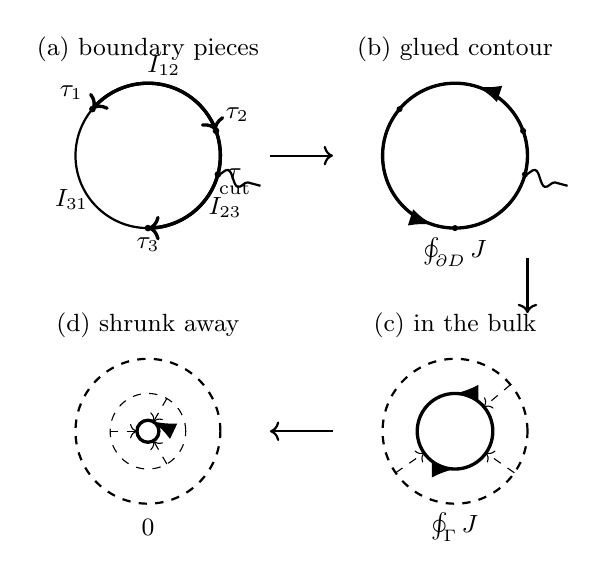
\begin{tikzpicture}[scale=1.0, every node/.style={font=\small}]
		% Top-left
		\begin{scope}[shift={(0,1.45)}]
			\node at (0,1.35) {(a) boundary pieces};
			\draw[thick] (0,0) circle (0.92);
			\fill (140:0.92) circle (1.2pt) node[above left] {$\tau_1$};
			\fill (20:0.92) circle (1.2pt) node[above right] {$\tau_2$};
			\fill (-90:0.92) circle (1.2pt) node[below] {$\tau_3$};
			\fill (-15:0.92) circle (1.2pt) node[right] {$\tau$};
			\draw[snake it, thick] (-15:0.92) -- (-15:1.48);
			\node at (1.10,-0.42) {\scriptsize cut};
			\draw[very thick,->] (140:0.92) arc[start angle=140,end angle=20,radius=0.92];
			\draw[very thick,->] (20:0.92) arc[start angle=20,end angle=-90,radius=0.92];
			\draw[very thick,->] (-90:0.92) arc[start angle=-90,end angle=140,radius=0.92];
			\node at (80:1.16) {$I_{12}$};
			\node at (-34:1.18) {$I_{23}$};
			\node at (210:1.12) {$I_{31}$};
		\end{scope}

		\draw[->,thick] (1.55,1.45) -- (2.35,1.45);

		% Top-right
		\begin{scope}[shift={(3.90,1.45)}]
			\node at (0,1.35) {(b) glued contour};
			\draw[thick] (0,0) circle (0.92);
			\fill (140:0.92) circle (1.1pt);
			\fill (20:0.92) circle (1.1pt);
			\fill (-90:0.92) circle (1.1pt);
			\fill (-15:0.92) circle (1.1pt);
			\draw[snake it, thick] (-15:0.92) -- (-15:1.48);
			\draw[very thick,postaction={decorate},
				decoration={markings,
					mark=at position 0.20 with {\arrow{Latex}},
					mark=at position 0.70 with {\arrow{Latex}}}]
				(0,0) circle (0.92);
			\node at (0,-1.22) {$\oint_{\partial D} J$};
		\end{scope}

		\draw[->,thick] (4.82,0.15) -- (4.82,-0.55);

		% Bottom-right
		\begin{scope}[shift={(3.90,-2.05)}]
			\node at (0,1.35) {(c) in the bulk};
			\draw[thick,dashed] (0,0) circle (0.92);
			\draw[very thick,postaction={decorate},
				decoration={markings,
					mark=at position 0.25 with {\arrow{Latex}},
					mark=at position 0.75 with {\arrow{Latex}}}]
				(0,0) circle (0.48);
			\foreach \ang in {40,-35,-145}{
				\draw[dashed,->] (\ang:0.92) -- (\ang:0.48);
			}
			\node at (0,-1.22) {$\oint_{\Gamma} J$};
		\end{scope}

		\draw[->,thick] (2.35,-2.05) -- (1.55,-2.05);

		% Bottom-left
		\begin{scope}[shift={(0,-2.05)}]
			\node at (0,1.35) {(d) shrunk away};
			\draw[thick,dashed] (0,0) circle (0.92);
			\draw[dashed] (0,0) circle (0.48);
			\draw[very thick,postaction={decorate},
				decoration={markings,
					mark=at position 0.18 with {\arrow{Latex}}}]
				(0,0) circle (0.14);
			\foreach \ang in {60,-60,180}{
				\draw[dashed,->] (\ang:0.48) -- (\ang:0.14);
			}
			\node at (0,-1.22) {$0$};
		\end{scope}
	\end{tikzpicture}
		\vspace{0.3em}
		\caption{Disk-level contour pulling in four steps. The three ordered boundary integrals are first glued into one contour on $\partial D$, then deformed into the bulk as a holomorphic contour $\Gamma$, and finally shrunk away because the interior contains no singularity for a massless integrated open-string insertion in the noncompact NCOS limit.}
		\label{fig:massless-decoupling-contour}
\end{figure}

Gomis and Ooguri recast the same decoupling mechanism in the first-order variables as a purely geometric statement on the doubled worldsheet \cite{gomis2000nonrelativisticclosedstringtheory}. Let $\Sigma_{g,h}$ denote an open worldsheet with $g$ handles and $h$ boundary components. Its Schottky double is obtained by taking a second copy with conjugate complex structure and gluing corresponding boundary points,
\ie\label{ncosschottkydouble}
\widehat\Sigma=\Sigma_{g,h}\cup_{\partial\Sigma}\overline{\Sigma}_{g,h},
\qquad
g(\widehat\Sigma)=2g+h-1.
\fe
The antiholomorphic involution exchanging the two copies fixes the glued circles $C_a$, which are precisely the original boundary components now viewed as interior cycles of the closed surface $\widehat\Sigma$. If one regards the original copy $\Sigma_{g,h}$ as a two-chain in $\widehat\Sigma$, then its boundary is literally the sum of those fixed cycles,
\ie\label{ncosboundarysum}
\partial[\Sigma_{g,h}]=[C_1]+\cdots+[C_h],
\qquad
[C_1+\cdots +C_h]=0\in H_1(\widehat\Sigma,\mathbb Z).
\fe
For a massless open-string insertion, the critical-field OPE implies that after choosing one lightcone chirality ($k_-=0$ or $k_+=0$) the integrated boundary vertex is the restriction of a holomorphic current $J(z)$ on $\widehat\Sigma$. Therefore the all-orders contour is not merely homologous to zero in the abstract sense: it is the boundary of the chosen half $\Sigma_{g,h}$, so
\ie\label{ncosholomorphicboundary}
\sum_{a=1}^h \oint_{C_a}J(z)
=\oint_{\partial\Sigma_{g,h}}J(z)
=0.
\fe
This is why the massless integrated vertex must be summed over all boundaries of the open diagram. Figure~\ref{fig:annulus-double} makes the contour pulling explicit for the annulus, Fig.~\ref{fig:schottky-double} shows the boundary-chain argument for general $(g,h)$, and Fig.~\ref{fig:schottky-gluing3d} gives a separate three-dimensional schematic of the gluing $\Sigma_{g,h}\cup_{\partial\Sigma}\overline\Sigma_{g,h}$ itself.

The local geometry of the doubling is simple. Near one boundary component choose a collar coordinate $w=\sigma+i\tau$ on $\Sigma_{g,h}$ with $\tau\ge0$. The conjugate copy carries the reflected collar $\bar w=\sigma-i\tau$, again with $\tau\ge0$ on its own sheet. Gluing corresponding boundary points means identifying the loci with the same $\sigma$ at $\tau=0$, so the two half-collars combine into a full neighborhood $-\epsilon<\tau<\epsilon$. The old boundary circle therefore ceases to be an edge of the surface and becomes an interior fixed cycle of the antiholomorphic involution $\tau\mapsto-\tau$.

To see explicitly how the disconnected cycles become a shrinkable contour, choose a cut graph $K\subset\Sigma_{g,h}$ that connects the boundary components and cuts the handles so that $\Sigma_{g,h}\setminus K$ is a disk. A thin neighborhood of $K\cup\partial\Sigma_{g,h}$ has a single connected boundary $\Gamma$ in the interior of the chosen half, and in homology
\ie\label{ncoscutgraphcontour}
[\Gamma]=[C_1]+\cdots+[C_h].
\fe
Because the current $J(z)$ is holomorphic and the interior contains no singularity, one may deform the original sum of boundary integrals to $\oint_\Gamma J$; after that, $\Gamma$ can be pushed across the disk $\Sigma_{g,h}\setminus K$ and shrunk away.

\begin{figure}[t]
	\centering
		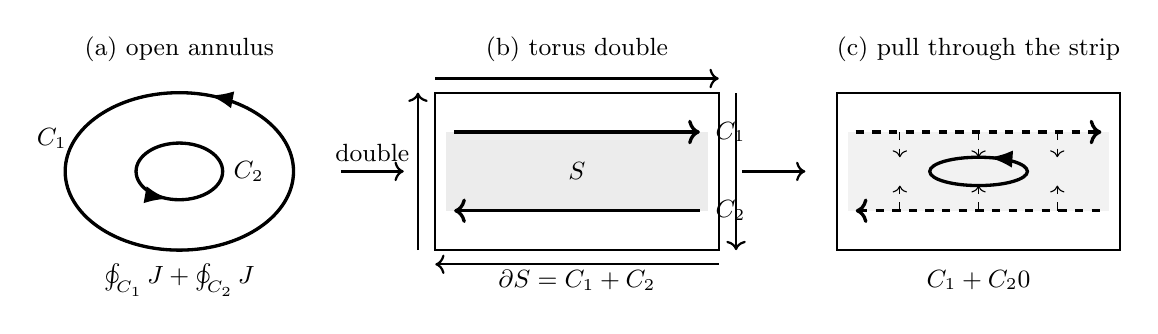
\begin{tikzpicture}[scale=1.0, every node/.style={font=\small}]
			% Panel (a): annulus
			\begin{scope}[shift={(0,0)}]
				\node at (0,1.55) {(a) open annulus};
				\draw[thick] (0,0) ellipse (1.45 and 1.00);
				\draw[thick] (0,0) ellipse (0.55 and 0.36);
				\draw[very thick,postaction={decorate},
					decoration={markings,mark=at position 0.20 with {\arrow{Latex}}}]
					(0,0) ellipse (1.45 and 1.00);
				\draw[very thick,postaction={decorate},
					decoration={markings,mark=at position 0.70 with {\arrow{Latex}}}]
					(0,0) ellipse (0.55 and 0.36);
				\node at (-1.62,0.42) {$C_1$};
				\node at (0.88,0.00) {$C_2$};
				\node at (0,-1.38) {$\oint_{C_1}J+\oint_{C_2}J$};
			\end{scope}

			\draw[->,thick] (2.05,0) -- (2.85,0) node[midway,above] {double};

			% Panel (b): torus double
			\begin{scope}[shift={(5.05,0)}]
				\node at (0,1.55) {(b) torus double};
				\draw[thick] (-1.80,-1.00) rectangle (1.80,1.00);
				\draw[->,thick] (-1.80,1.18) -- (1.80,1.18);
				\draw[<-,thick] (-1.80,-1.18) -- (1.80,-1.18);
				\draw[->,thick] (-2.02,-1.00) -- (-2.02,1.00);
				\draw[<-,thick] (2.02,-1.00) -- (2.02,1.00);
				\fill[gray!15] (-1.66,-0.50) rectangle (1.66,0.50);
				\draw[very thick,->] (-1.56,0.50) -- (1.56,0.50);
				\draw[very thick,<-] (-1.56,-0.50) -- (1.56,-0.50);
				\node at (1.95,0.50) {$C_1$};
				\node at (1.95,-0.50) {$C_2$};
				\node at (0,0.00) {$S$};
				\node at (0,-1.38) {$\partial S=C_1+C_2$};
			\end{scope}

			\draw[->,thick] (7.15,0) -- (7.95,0);

			% Panel (c): pulled through strip
			\begin{scope}[shift={(10.15,0)}]
				\node at (0,1.55) {(c) pull through the strip};
				\draw[thick] (-1.80,-1.00) rectangle (1.80,1.00);
				\fill[gray!10] (-1.66,-0.50) rectangle (1.66,0.50);
				\draw[dashed,very thick,->] (-1.56,0.50) -- (1.56,0.50);
				\draw[dashed,very thick,<-] (-1.56,-0.50) -- (1.56,-0.50);
				\foreach \x in {-1.0,0.0,1.0}{
					\draw[dashed,->] (\x,0.50) -- (\x,0.18);
					\draw[dashed,->] (\x,-0.50) -- (\x,-0.18);
				}
				\draw[very thick,postaction={decorate},
					decoration={markings,mark=at position 0.20 with {\arrow{Latex}}}]
					(0,0) ellipse (0.62 and 0.18);
				\node at (0,-1.38) {$C_1+C_2 \rightsquigarrow 0$};
			\end{scope}
		\end{tikzpicture}
		\vspace{0.2em}
		\caption{Contour pulling for the first nontrivial all-orders example. On the annulus the two boundary components carry opposite induced orientations; after doubling, their sum bounds the strip $S$ on the torus, so the paired contour can be pushed through $S$ and removed.}
		\label{fig:annulus-double}
\end{figure}

\begin{figure}[t]
	\centering
		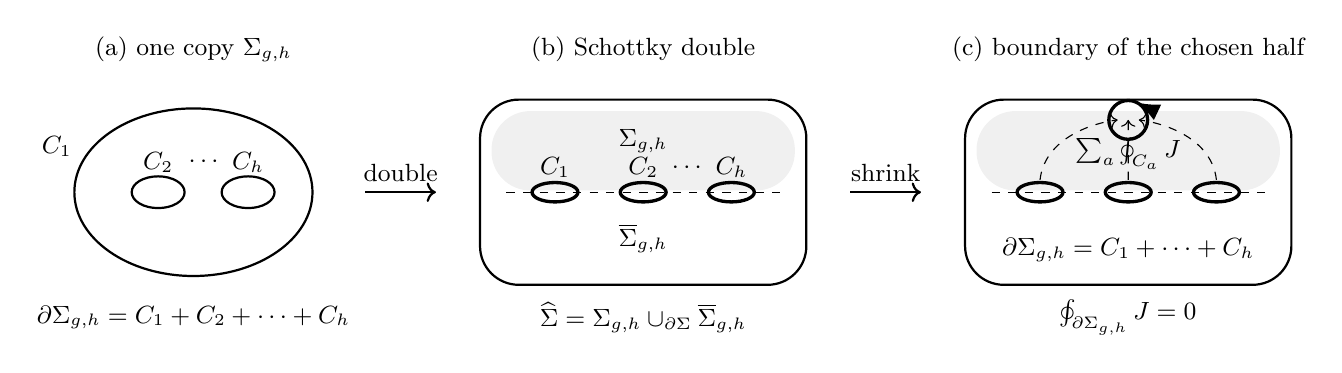
\begin{tikzpicture}[scale=1.12, every node/.style={font=\small}]
			% Panel (a): open surface
			\begin{scope}[shift={(0,0)}]
				\node at (0,1.62) {(a) one copy $\Sigma_{g,h}$};
				\draw[thick] (0,0) ellipse (1.35 and 0.95);
				\draw[thick] (-0.40,0) ellipse (0.30 and 0.18);
				\draw[thick] (0.62,0) ellipse (0.30 and 0.18);
				\node at (-1.55,0.52) {$C_1$};
				\node at (-0.40,0.34) {$C_2$};
				\node at (0.62,0.34) {$C_h$};
				\node at (0.14,0.34) {$\cdots$};
				\node at (0,-1.42) {$\partial\Sigma_{g,h}=C_1+C_2+\cdots +C_h$};
			\end{scope}

			\draw[->,thick] (1.95,0) -- (2.75,0) node[midway,above] {double};

			% Panel (b): Schottky double
			\begin{scope}[shift={(5.10,0)}]
				\node at (0,1.62) {(b) Schottky double};
				\draw[thick, rounded corners=14pt] (-1.85,-1.05) rectangle (1.85,1.05);
				\fill[gray!12, rounded corners=14pt] (-1.72,0.02) rectangle (1.72,0.92);
				\draw[dashed] (-1.55,0) -- (1.55,0);
				\draw[very thick] (-1.00,0) ellipse (0.26 and 0.11);
				\draw[very thick] (0.00,0) ellipse (0.26 and 0.11);
				\draw[very thick] (1.00,0) ellipse (0.26 and 0.11);
				\node at (-1.00,0.28) {$C_1$};
				\node at (0.00,0.28) {$C_2$};
				\node at (1.00,0.28) {$C_h$};
				\node at (0.52,0.28) {$\cdots$};
				\node at (0,0.58) {$\Sigma_{g,h}$};
				\node at (0,-0.52) {$\overline{\Sigma}_{g,h}$};
				\node at (0,-1.42) {$\widehat\Sigma=\Sigma_{g,h}\cup_{\partial\Sigma}\overline{\Sigma}_{g,h}$};
			\end{scope}

			\draw[->,thick] (7.45,0) -- (8.25,0) node[midway,above] {shrink};

			% Panel (c): contour shrinking
			\begin{scope}[shift={(10.60,0)}]
				\node at (0,1.62) {(c) boundary of the chosen half};
				\draw[thick, rounded corners=14pt] (-1.85,-1.05) rectangle (1.85,1.05);
				\fill[gray!12, rounded corners=14pt] (-1.72,0.02) rectangle (1.72,0.92);
				\draw[dashed] (-1.55,0) -- (1.55,0);
				\draw[very thick] (-1.00,0) ellipse (0.26 and 0.11);
				\draw[very thick] (0.00,0) ellipse (0.26 and 0.11);
				\draw[very thick] (1.00,0) ellipse (0.26 and 0.11);
				\draw[dashed,->] (-1.00,0.14) .. controls (-0.95,0.59) and (-0.45,0.78) .. (-0.12,0.82);
				\draw[dashed,->] (0.00,0.14) .. controls (0.00,0.51) and (0.00,0.70) .. (0.00,0.82);
				\draw[dashed,->] (1.00,0.14) .. controls (0.95,0.59) and (0.45,0.78) .. (0.12,0.82);
				\draw[very thick,postaction={decorate},
					decoration={markings,mark=at position 0.18 with {\arrow{Latex}}}]
					(0,0.82) circle (0.22);
				\node at (0,0.44) {$\sum_a \oint_{C_a}J$};
				\node at (0,-0.66) {$\partial\Sigma_{g,h}=C_1+\cdots +C_h$};
				\node at (0,-1.42) {$\oint_{\partial\Sigma_{g,h}}J=0$};
			\end{scope}
		\end{tikzpicture}
		\vspace{0.2em}
		\caption{Schottky doubling and the all-orders contour argument. Doubling $\Sigma_{g,h}$ glues it to its mirror and turns the old boundary components into fixed cycles of $\widehat\Sigma$. Their sum is the actual boundary of the chosen half, $\partial\Sigma_{g,h}=C_1+\cdots +C_h$, so the summed massless contour is a genuine boundary contour and can be shrunk away. Extra handles of $\widehat\Sigma$ are suppressed in this schematic.}
		\label{fig:schottky-double}
\end{figure}

\clearpage
\begin{center}
\begin{minipage}{\linewidth}
	\centering
		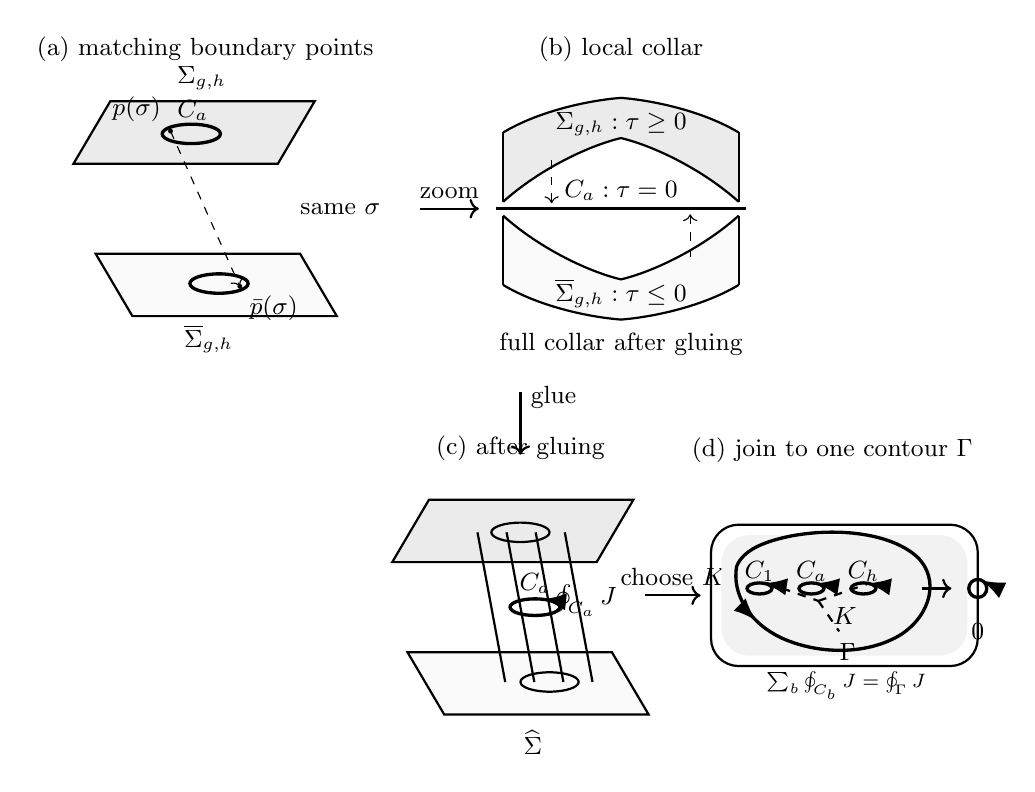
\begin{tikzpicture}[scale=0.88, every node/.style={font=\small}]
			% Panel (a): copy and conjugate copy
			\begin{scope}[shift={(0,0)}]
				\node at (0,2.30) {(a) matching boundary points};

				\fill[gray!16] (-1.90,0.65) -- (1.05,0.65) -- (1.58,1.55) -- (-1.37,1.55) -- cycle;
				\draw[thick] (-1.90,0.65) -- (1.05,0.65) -- (1.58,1.55) -- (-1.37,1.55) -- cycle;
				\draw[very thick] (-0.20,1.08) ellipse (0.42 and 0.14);
				\fill (-0.50,1.12) circle (1.0pt);
				\node[above left] at (-0.50,1.12) {$p(\sigma)$};
				\node at (-0.18,1.42) {$C_a$};
				\node at (-0.05,1.88) {$\Sigma_{g,h}$};

				\fill[gray!4] (-1.05,-1.55) -- (1.90,-1.55) -- (1.37,-0.65) -- (-1.58,-0.65) -- cycle;
				\draw[thick] (-1.05,-1.55) -- (1.90,-1.55) -- (1.37,-0.65) -- (-1.58,-0.65) -- cycle;
				\draw[very thick] (0.20,-1.08) ellipse (0.42 and 0.14);
				\fill (0.50,-1.12) circle (1.0pt);
				\node[below right] at (0.50,-1.12) {$\bar p(\sigma)$};
				\node at (0.05,-1.88) {$\overline{\Sigma}_{g,h}$};

				\draw[dashed,->] (-0.50,1.12) -- (0.50,-1.12);
				\node at (1.95,0.00) {\small same $\sigma$};
			\end{scope}

			\draw[->,thick] (3.10,0.00) -- (3.95,0.00) node[midway,above] {zoom};

			% Panel (b): local collar model
			\begin{scope}[shift={(6.00,0)}]
				\node at (0,2.30) {(b) local collar};
				\fill[gray!16] (-1.70,0.10) .. controls (-1.20,0.55) and (-0.50,0.90) .. (0.00,1.02)
					.. controls (0.50,0.90) and (1.20,0.55) .. (1.70,0.10)
					-- (1.70,1.10) .. controls (1.20,1.40) and (0.50,1.56) .. (0.00,1.60)
					.. controls (-0.50,1.56) and (-1.20,1.40) .. (-1.70,1.10) -- cycle;
				\draw[thick] (-1.70,0.10) .. controls (-1.20,0.55) and (-0.50,0.90) .. (0.00,1.02)
					.. controls (0.50,0.90) and (1.20,0.55) .. (1.70,0.10);
				\draw[thick] (-1.70,1.10) .. controls (-1.20,1.40) and (-0.50,1.56) .. (0.00,1.60)
					.. controls (0.50,1.56) and (1.20,1.40) .. (1.70,1.10);
				\draw[thick] (-1.70,0.10) -- (-1.70,1.10);
				\draw[thick] (1.70,0.10) -- (1.70,1.10);

				\fill[gray!4] (-1.70,-0.10) .. controls (-1.20,-0.55) and (-0.50,-0.90) .. (0.00,-1.02)
					.. controls (0.50,-0.90) and (1.20,-0.55) .. (1.70,-0.10)
					-- (1.70,-1.10) .. controls (1.20,-1.40) and (0.50,-1.56) .. (0.00,-1.60)
					.. controls (-0.50,-1.56) and (-1.20,-1.40) .. (-1.70,-1.10) -- cycle;
				\draw[thick] (-1.70,-0.10) .. controls (-1.20,-0.55) and (-0.50,-0.90) .. (0.00,-1.02)
					.. controls (0.50,-0.90) and (1.20,-0.55) .. (1.70,-0.10);
				\draw[thick] (-1.70,-1.10) .. controls (-1.20,-1.40) and (-0.50,-1.56) .. (0.00,-1.60)
					.. controls (0.50,-1.56) and (1.20,-1.40) .. (1.70,-1.10);
				\draw[thick] (-1.70,-0.10) -- (-1.70,-1.10);
				\draw[thick] (1.70,-0.10) -- (1.70,-1.10);

				\draw[very thick] (-1.80,0) -- (1.80,0);
				\draw[dashed,->] (-1.00,0.70) -- (-1.00,0.08);
				\draw[dashed,->] (1.00,-0.70) -- (1.00,-0.08);
				\node at (0,0.26) {$C_a:\tau=0$};
				\node at (0,1.22) {$\Sigma_{g,h}:\tau\ge0$};
				\node at (0,-1.22) {$\overline{\Sigma}_{g,h}:\tau\le0$};
				\node at (0,-1.95) {full collar after gluing};
			\end{scope}

			\draw[->,thick] (4.55,-2.65) -- (4.55,-3.55) node[pos=0.08,right] {glue};

			% Panel (c): glued surface
			\begin{scope}[shift={(4.55,-5.75)}]
				\node at (0,2.30) {(c) after gluing};

				\fill[gray!16] (-1.85,0.65) -- (1.10,0.65) -- (1.63,1.55) -- (-1.32,1.55) -- cycle;
				\draw[thick] (-1.85,0.65) -- (1.10,0.65) -- (1.63,1.55) -- (-1.32,1.55) -- cycle;
				\fill[gray!4] (-1.10,-1.55) -- (1.85,-1.55) -- (1.32,-0.65) -- (-1.63,-0.65) -- cycle;
				\draw[thick] (-1.10,-1.55) -- (1.85,-1.55) -- (1.32,-0.65) -- (-1.63,-0.65) -- cycle;

				\draw[thick] (-0.62,1.08) -- (-0.22,-1.08);
				\draw[thick] (0.22,1.08) -- (0.62,-1.08);
				\draw[thick] (-0.20,1.08) -- (0.20,-1.08);
				\draw[thick] (0.64,1.08) -- (1.04,-1.08);

				\draw[thick] (0.00,1.08) ellipse (0.42 and 0.14);
				\draw[thick] (0.42,-1.08) ellipse (0.42 and 0.14);
				\draw[very thick,postaction={decorate},
					decoration={markings,mark=at position 0.18 with {\arrow{Latex}}}]
					(0.21,0.00) ellipse (0.36 and 0.12);
				\node at (0.21,0.34) {$C_a$};
				\node at (0.95,0.10) {$\oint_{C_a}J$};
				\node at (0.18,-1.95) {$\widehat\Sigma$};
			\end{scope}

			\draw[->,thick] (6.35,-5.58) -- (7.15,-5.58) node[midway,above] {choose $K$};

			% Panel (d): the disconnected cycles join through a cut graph
			\begin{scope}[shift={(9.05,-5.58)}, every node/.style={font=\small}]
				\node at (0,2.10) {(d) join to one contour $\Gamma$};
				\draw[thick,rounded corners=10pt] (-1.75,-1.02) rectangle (2.10,1.02);
				\fill[gray!10,rounded corners=10pt] (-1.60,-0.87) rectangle (1.95,0.87);

				% seam circles
				\draw[very thick,postaction={decorate},
					decoration={markings,mark=at position 0.18 with {\arrow{Latex}}}]
					(-1.05,0.10) ellipse (0.18 and 0.08);
				\draw[very thick,postaction={decorate},
					decoration={markings,mark=at position 0.18 with {\arrow{Latex}}}]
					(-0.30,0.10) ellipse (0.18 and 0.08);
				\draw[very thick,postaction={decorate},
					decoration={markings,mark=at position 0.18 with {\arrow{Latex}}}]
					(0.45,0.10) ellipse (0.18 and 0.08);
				\node at (-1.05,0.34) {$C_1$};
				\node at (-0.30,0.34) {$C_a$};
				\node at (0.45,0.34) {$C_h$};

				% cut graph and connected contour around its neighborhood
				\draw[dashed,thick] (-0.95,0.18) -- (-0.20,-0.08);
				\draw[dashed,thick] (-0.20,-0.08) -- (0.55,0.18);
				\draw[dashed,thick] (-0.20,-0.08) -- (0.10,-0.52);
				\node at (0.18,-0.30) {$K$};
				\draw[very thick,postaction={decorate},
					decoration={markings,mark=at position 0.12 with {\arrow{Latex}}}]
					(-1.38,0.42) .. controls (-1.45,0.02) and (-1.20,-0.40) .. (-0.72,-0.62)
					.. controls (-0.18,-0.86) and (0.52,-0.86) .. (1.00,-0.56)
					.. controls (1.42,-0.28) and (1.56,0.24) .. (1.22,0.56)
					.. controls (0.84,0.90) and (0.08,0.98) .. (-0.58,0.86)
					.. controls (-0.98,0.78) and (-1.28,0.66) .. (-1.38,0.42);
				\node at (0.22,-0.82) {$\Gamma$};

				\draw[->,thick] (1.30,0.10) -- (1.72,0.10);
				\draw[very thick,postaction={decorate},
					decoration={markings,mark=at position 0.18 with {\arrow{Latex}}}]
					(2.10,0.10) ellipse (0.13 and 0.13);
				\node at (2.10,-0.52) {$0$};
				\node[font=\scriptsize] at (0.20,-1.30) {$\sum_b \oint_{C_b}J=\oint_\Gamma J$};
			\end{scope}
		\end{tikzpicture}
		\vspace{0.05em}
		\captionsetup{hypcap=false}
		\captionof{figure}{Three-dimensional Schottky double and contour joining. After gluing, choose a cut graph $K\subset\Sigma_{g,h}$ in the chosen half; the contour $\Gamma$ around a thin neighborhood of $K\cup\partial\Sigma_{g,h}$ is connected, homologous to $C_1+\cdots +C_h$, and shrinks to zero.}
		\label{fig:schottky-gluing3d}
\end{minipage}
\end{center}

This also clarifies the limitations of the argument. For a massive integrated open-string leg the boundary operator depends on both chiralities, so it is not the restriction of a holomorphic current on $\widehat\Sigma$ and the contour cannot be deformed away. Likewise, if $x^1$ is compact, wound closed strings exist and the ``no bulk insertion'' step of the noncompact proof fails. The all-orders U$(1)$ decoupling statement is therefore special to the noncompact 1+1 NCOS limit with at least one massless open-string insertion.

\subsection{Connection to 2D SYM flux sectors}
We now connect the NCOS/BCFT data above to the dual 2D SYM description. In the holographic map, (\ref{ncoslimit}) is not an independent gauge-theory limit; in SYM variables the relevant scaling is
\ie\label{symncoslimit}
E\sim {g_{\rm YM}\over N},~~~~g_{\rm YM}~{\rm fixed},~~~~k=1~{\rm flux~sector},
\fe
namely we focus on the flux-sector states at this energy scale (rather than taking a strict $N\to\infty$ limit), and use the corresponding $1/N$ asymptotic expansion. The near-critical behavior then follows from flux quantization below.
More generally, the SYM superselection sector is labeled by $k\in\mathbb{Z}_N$ electric flux units, with ground-state energy density
\ie\label{symfluxenergy}
E_k=\,{k^2 g_{\rm YM}^2\over 2N},
\fe
as in \cite{cho2026fluxsectorsmatrixstring} (equation (2.1) there). In the diagonal $U(1)$ description this is equivalently a constant flux density $F_{01}^{\rm diag}=k g_{\rm YM}^2/N$. Under the NCOS/SYM map, $k$ is identified with the number $M$ of D1-branes in the NCOS frame.


Having derived the BCFT and scaling data in the parent D1$+$flux system, we now map it into the holographic channel (\ref{dsaiibdoness}), (\ref{f1sdualbg}), which are already near-horizon geometries. The flux-sector interpretation follows directly from the D1/F1 dual pair: in the D1 frame, F1 charge is realized as electric world volume flux on the D1; in the S-dual frame this is described by a D1 probe in the F1 background (\ref{f1sdualbg}), with the original D1 charge of (\ref{dsaiibdoness}) mapped to dissolved F1 charge in the probe D1 world volume field. This is the same $(p,q)$-string bound-state mechanism that underlies the 1+1 NCOS/SYM dictionary \cite{gopakumar2000sdualitynoncommutativegaugetheory,klebanov200011dimensionalncosun,yin2026foundationsofstringtheory}; see in particular equations (2.4), (2.5), (3.4) of \cite{gopakumar2000sdualitynoncommutativegaugetheory} and equations (1), (2), (3) of \cite{klebanov200011dimensionalncosun}. For Xi's derivation, see chapter 18 equations (18.50), (18.53), (18.54), (18.57), (18.58).

It is worth emphasizing that the near-critical electric-field scaling $\widetilde E\to 1$ in the S-dual description is not an independent limit: holding $\A'_{\rm eff}$ and $G_o$ fixed implies $G_o^4\A'_{\rm eff}=\wt g_B^{\,2}\wt\ell_B^{\,2}=\ell_B^2/g_B$ (using $\wt g_B=g_B^{-1}$ and $\wt\ell_B^2=g_B\ell_B^2$), so equivalently $g_B/\ell_B^2$ (and hence $g_{\rm YM}^2$) is fixed in the original D1 decoupling limit.

For the single-flux sector on the SYM side ($k=1$), equivalently one D1-brane on the NCOS side ($M=1$) carrying $N$ electric-flux units, the normalizations can be derived directly in Xi's conventions \cite{yin2026foundationsofstringtheory} (chapter 18 equations (18.50), (18.53), (18.54)). For constant electric field and vanishing RR axion, the D1 Born-Infeld Lagrangian density is
\ie\label{d1dbisingleflux}
{\cal L}_{\rm D1}=-{1\over 2\pi \wt\ell_B^2 \wt g_B}\sqrt{1-\widetilde E^2},
\fe
Upon compactifying $x\sim x+2\pi R$, canonical momentum quantization gives
\ie\label{singlefluxquant}
\Pi_{A_1}=2\pi R\,{\widetilde E\over \wt g_B\sqrt{1-\widetilde E^2}}=2\pi N R
~~\Longrightarrow~~
N={\widetilde E\over \wt g_B\sqrt{1-\widetilde E^2}}.
\fe
Equivalently,
\ie\label{efluxsolve}
\widetilde E={N\wt g_B\over \sqrt{1+N^2\wt g_B^2}}
=\left(1+{1\over N^2\wt g_B^2}\right)^{-{1\over 2}} = \left(1+\frac{2\pi g_{\rm YM}^2 \wt{\ell}_B^2}{N^2}\right)^{-{1\over 2}}.
\fe
At the energy scale
\be
\frac{g_{\rm YM}}{N} \ll \frac{1}{\wt{\ell}_B},
\ee
we effectively have $\wt{E} \to 1$.
This makes the SYM interpretation explicit: the dual $U(N)$ theory is in a discrete electric-flux superselection sector (single-flux case here), and $\widetilde E$ is fixed by that sector and couplings rather than being an independent continuous SYM control parameter \cite{klebanov200011dimensionalncosun,cho2026fluxsectorsmatrixstring}.
Combining (\ref{singlefluxquant}) with the BCFT coupling and tension formulas above gives
\ie\label{gzeroderive}
G_o^2={\widetilde E\over N}
\to {1\over N},
\fe
\ie\label{alphaeffderivea}
\A'_{\rm eff}={\wt\ell_B^2\wt g_B^2 N^2\over \widetilde E^2}
\;
\to \wt\ell_B^2\wt g_B^2N^2 = \frac{N^2}{2\pi g_{\rm YM}^2},
\fe
which is the single-flux NCOS/SYM dictionary (equivalent to the one in \cite{klebanov200011dimensionalncosun}, equations (1), (2), (3), after converting conventions). The condition $\wt{E} \to 1$ means a hierarchy of tensions $\frac{1}{\A'_{\rm eff}} \ll \frac{1}{\wt{\alpha}'_B}$.
Crucially, this is not a truncation of the open-string tower: open-string oscillator states at $m^2\sim 1/\A'_{\rm eff} \sim \frac{g_{\rm YM}^2}{N^2}$ remain in the NCOS spectrum.

\subsubsection{Holographic route from the compact D1 throat to NRCS}
\noindent
The question here is narrower than the full SYM/string duality: starting from the compactified background (\ref{f1sdualbg}), is one really looking at NRCS? The answer is no globally, but yes locally after T-duality and freezing the radial variation. The derivation is completely at the level of background fields.

Compactify the spatial direction of the D1 system as
\ie\label{mscompactx}
x\sim x+2\pi R.
\fe
Setting the electric-flux label of (\ref{symfluxenergy}) to $k=0$ removes the NCOS probe/open-string sector, but it does {\it not} remove the rank-$N$ holographic system itself: the same D1 charge $N$ in (\ref{dsaiibdoness}) still labels the dual $U(N)$ gauge theory. Now apply standard Buscher T-duality along the compact $x$-circle directly to the S-dual F1 background (\ref{f1sdualbg}). Since
\ie
g_{tt}=-\wt f_1(r)^{-1},\qquad
g_{xx}=\wt f_1(r)^{-1},\qquad
B_{tx}=\wt f_1(r)^{-1},
\fe
the T-dual type-IIA background is
\ie\label{iiappcompact}
ds_{\rm str}^2
=
2\,dt\,d\wt x
+\wt f_1(r)\,d\wt x^2
+dr^2+r^2d\Omega_7^2,
\qquad
\wt x\sim \wt x+2\pi{\A'_A\over R},
\fe
\ie\label{iiappparams}
e^{\Phi_A}=1,
\qquad
\A'_A\equiv \ell_A^2=\wt\ell_B^2,
\qquad
g_A=\wt g_B\,{\wt\ell_B\over R}
=
{1\over \sqrt{2\pi}\,g_{\rm YM}R}.
\fe
Here $\A'_A$ is the type-IIA string scale. No matrix-string input has entered yet: (\ref{iiappcompact}) is just the exact T-dual bulk geometry of the compact near-horizon F1 throat.

This is also the right place to compare with section 3.2 of Danielsson, Guijosa, and Kruczenski \cite{danielsson2000iiabwoundwrapped}, titled ``$B$ is for Boost.'' Their point is that for a {\it flat} compact background with constant $B_{01}$, Buscher duality converts the $B$-field into an off-diagonal metric, and a further linear change of coordinates brings that metric to the frame of a boosted background with $B=0$. Writing
\ie\label{boostvelocitydef}
v\equiv 2\pi\A' B_{01},
\qquad
\gamma_{\rm boost}\equiv (1-v^2)^{-1/2},
\fe
the flat T-dual longitudinal metric takes the form
\ie\label{boostmetricflat}
ds^2_{01}
=
-(1-v^2)(dX^0)^2
+2v\,dX^0d\wt X^1
+(d\wt X^1)^2,
\fe
which is the version of equation (3.10) in \cite{danielsson2000iiabwoundwrapped} written in our dimensionful coordinates. Section 3.2 then shows that after passing to the coordinates of the boosted frame, the same background is just flat space with $B=0$ and a compact circle that is not aligned with the original time slice. In that precise sense a constant $B_{01}$ and a boost are equivalent descriptions of the same compact flat problem. The equivalence is not the statement that a Lorentz boost changes the local supergravity fields of a curved F1 throat. Rather, the boost interpretation appears only after T-duality and after choosing coordinates adapted to the compact identification.

Equation (\ref{iiappcompact}) already shows why (\ref{f1sdualbg}) is not globally the Gomis-Ooguri background. The coefficient of $d\wt x^2$ is $\wt f_1(r)$, so it varies with the transverse position, and the transverse metric is the curved eight-dimensional cone $dr^2+r^2d\Omega_7^2$ rather than flat $\bR^8$ with a single fixed scale $\A'_{\rm eff}$. So there is no exact global identification of (\ref{f1sdualbg}) with the flat NRCS parent background.

To compare with Gomis-Ooguri, recall their flat parent background after T-duality along the compact longitudinal circle. Starting from
\ie
ds^2=-(dX^0)^2+(dX^1)^2+g_{ij}\,dX^i dX^j,
\qquad
2\pi\A' B_{01}=1-{\A'\over 2\A'_{\rm eff}},
\fe
Buscher duality along $X^1$ gives the exact two-dimensional longitudinal metric \cite{gomis2000nonrelativisticclosedstringtheory}
\ie\label{gotdualmetric}
ds^2_{01}
=
\left[-1+\left(2\pi\A' B_{01}\right)^2\right](dX^0)^2
+2\left(2\pi\A' B_{01}\right)dX^0 d\wt X^1
+(d\wt X^1)^2.
\fe
Equivalently, after the definition (\ref{boostvelocitydef}),
\ie
ds^2_{01}
=
-(1-v^2)(dX^0)^2
+2v\,dX^0d\wt X^1
+(d\wt X^1)^2.
\fe
In the strict critical endpoint $2\pi\A' B_{01}=1$, this reduces to
\ie\label{gocriticaltdual}
ds^2_{01}=2\,dX^0 d\wt X^1+(d\wt X^1)^2.
\fe
This is the background-level form that underlies the Gomis-Ooguri first-order rewrite. It is also the flat-space version of the Danielsson-Guijosa-Kruczenski statement: after T-duality, the near-critical $B_{01}$ background is rewritten as the off-diagonal metric (\ref{boostmetricflat}), with boost parameter $v=2\pi\A' B_{01}$. The critical Gomis-Ooguri background (\ref{gocriticaltdual}) is the endpoint $v\to 1$, where the boosted compact direction becomes null.

Now freeze the radial coordinate of (\ref{iiappcompact}) at $r=r_\ast$ and work in a worldsheet patch small compared with the radial variation scale of $\wt f_1(r)$. Write $\wt f_1(r_\ast)\equiv H_\ast$, introduce local Cartesian transverse coordinates $y^i$, and define
\ie\label{tdual-local-coords}
t_{\rm loc}\equiv H_\ast^{-{1\over 2}}t,\qquad
\wt x_{\rm loc}\equiv H_\ast^{{1\over 2}}\wt x,\qquad
y^i_{\rm loc}\equiv H_\ast^{{1\over 2}}y^i.
\fe
Then the T-dual background becomes
\ie\label{f1localtdual}
ds_{\rm str}^2
\simeq
2\,dt_{\rm loc}\,d\wt x_{\rm loc}
+(d\wt x_{\rm loc})^2
+H_\ast^{-1}\delta_{ij}\,dy^i_{\rm loc}dy^j_{\rm loc},
\fe
up to derivative corrections suppressed by the local variation of $\wt f_1$. Comparing (\ref{f1localtdual}) with (\ref{gocriticaltdual}), one sees that the compactified T-dual throat is locally {\it exactly} the critical T-dual Gomis-Ooguri background, with local effective slope
\ie\label{localalphaefftdual}
\A'_{\rm eff}(r_\ast)\equiv \A'_A H_\ast,
\qquad
g_{ij}={\A'_A\over \A'_{\rm eff}(r_\ast)}\delta_{ij}=H_\ast^{-1}\delta_{ij}.
\fe
In the present near-horizon throat $H_\ast=\wt f_1(r_\ast)=c_1N/r_\ast^6$, so the exact radial dependence is
\ie\label{localalphaeffexact}
\A'_{\rm eff}(r)
=
\A'_A\,\wt f_1(r)
=
\A'_A{c_1N\over r^6}.
\fe
Using $\A'_A=\wt\ell_B^2$ and $c_1=32\pi^2\wt g_B^2\wt\ell_B^6$, this may also be written as
\ie
\A'_{\rm eff}(r)
=
32\pi^2\wt g_B^2 N\,{\wt\ell_B^8\over r^6}.
\fe
This is the precise sense in which the throat knows about NRCS. The curved background is the $r$-dependent analogue of the flat off-diagonal metric discussed in section 3.2 of \cite{danielsson2000iiabwoundwrapped}: each sufficiently small patch at fixed $r$ is equivalent to a constant-$B$ flat background and hence to the critical Gomis-Ooguri form, but there is no single global boost that removes the full $r$-dependence of (\ref{iiappcompact}).

The same background also gives the local string scale directly. Using (\ref{gymdict}) and (\ref{iiappparams}),
\ie
g_{\rm YM}^2={1\over 2\pi \wt g_B^2\wt\ell_B^2},
\qquad
c_1
=
32\pi^2\wt g_B^2\wt\ell_B^6
=
16\pi\,{\wt\ell_B^4\over g_{\rm YM}^2}.
\fe
Substituting this into (\ref{localalphaeffexact}) gives the exact bulk expression
\ie\label{alphaefffrom14}
\A'_{\rm eff}(r)
=
\A'_A\,\wt f_1(r)
=
16\pi\,{N\wt\ell_B^6\over g_{\rm YM}^2\,r^6}.
\fe
Now define the redshifted local type-IIA string scale by
\ie\label{redshiftedlocale}
E_{\rm string}(r)
\equiv
\sqrt{-g_{tt}(r)}\,{1\over \sqrt{\A'_A}}
=
\wt f_1(r)^{-{1\over 2}}\,{1\over \sqrt{\A'_A}}
=
{1\over \sqrt{\A'_{\rm eff}(r)}}.
\fe
Here $E_{\rm string}(r)$ means the energy, measured with respect to the asymptotic time $t$, of a local excitation at the type-IIA string scale. Using (\ref{alphaefffrom14}) this may be written as
\ie\label{redshiftedlocalexact}
E_{\rm string}(r)
=
{g_{\rm YM}\over 4\sqrt{\pi N}}
\left({r\over \wt\ell_B}\right)^3.
\fe
Equations (\ref{alphaefffrom14})--(\ref{redshiftedlocalexact}) are the direct output of the background (\ref{f1sdualbg}) and the local T-dual GO identification: they show that the throat itself furnishes an $r$-dependent family of string scales, or equivalently
\ie
\A'_{\rm eff}(r)=E_{\rm string}(r)^{-2}.
\fe
To turn this into a statement about the dual SYM one must specify which boundary energy scale is being matched to the bulk radius. If one matches to the single-flux sector scale $E\sim g_{\rm YM}/N$, then (\ref{redshiftedlocale}) immediately gives
\ie
\A'_{\rm eff}\sim {N^2\over g_{\rm YM}^2}.
\fe
This reproduces the NCOS/SYM scaling. The exact coefficient $1/(2\pi)$ in (\ref{alphaeffderivea}) is not fixed by (\ref{f1sdualbg}) alone; it comes from the probe/open-string normalization derived earlier.

To recover the usual Gomis-Ooguri first-order action, one now applies the inverse Buscher map back to the local constant-$B$ frame and then performs the standard first-order rewrite imported in (\ref{gomisgooguriaction}). Because all background fields are constant on the chosen patch, that local worldsheet action is exactly the Gomis-Ooguri action with $\A'_{\rm eff}$ replaced by the local value $\A'_{\rm eff}(r_\ast)$.

The resulting chain is
\ie\label{nrcssymchain}
\text{compact D1 near-horizon holography}
\;\Longrightarrow\;
{\rm compactified\ F1\ throat}\ (\ref{f1sdualbg})
\;\Longrightarrow\;
{\rm exact\ T\text{-}dual\ background}\ (\ref{iiappcompact})
\;\Longleftrightarrow\;
{\rm local\ critical\ GO/NRCS\ background}\ (\ref{f1localtdual}).
\fe
So the statement at the level of (\ref{f1sdualbg}) is sharp: it is {\it not} globally dual to NRCS, because the geometry is curved and $r$-dependent, but after compactifying $x$ and T-dualizing it becomes a curved family of local patches whose tangent-frame form is exactly the critical T-dual Gomis-Ooguri background. That is how the NRCS sector is extracted from (\ref{f1sdualbg}).

\subsection{Decoupling of closed strings}

The decoupling above is from bulk closed strings (and hence gravity), not from high open-string modes. A field-theory sector appears only after an additional IR restriction $E_{\rm phys}\ll 1/\sqrt{\A'_{\rm eff}}$.

For non-compact flat $x$, the closed-channel momentum along $x$ is continuous. At fixed closed-string oscillator level $N_{\rm cl}$ and fixed transverse momentum, define
\[
\Delta_{N_{\rm cl}}(\omega)\equiv M_{N_{\rm cl}}^2(\widetilde E,p_\perp)-\omega^2-i0,
\]
with
\[
M_{N_{\rm cl}}^2(\widetilde E,p_\perp)
=p_1^2+{p_\perp^2\over 1-\widetilde E^2}
 +{4(N_{\rm cl}-a_{\rm cl})\over \A'_{\rm eff}(1-\widetilde E^2)}.
\]
Then
\[
\mathcal A_{N_{\rm cl}}(\omega)\sim
\int_{-\infty}^{\infty}{dq_x\over q_x^2+\Delta_{N_{\rm cl}}(\omega)}
=\pi\,\Delta_{N_{\rm cl}}(\omega)^{-1/2},
\]
so the singularity is a threshold branch point rather than an isolated pole:
\[
{\rm Disc}\,\mathcal A_{N_{\rm cl}}(\omega)\propto
{\theta\!\left(\omega^2-M_{N_{\rm cl}}^2\right)\over
\sqrt{\omega^2-M_{N_{\rm cl}}^2}}.
\]
The non-planar Moyal factor enters in the open channel as $e^{ib(\theta,p)q_x}$; after Gaussian integration,
\[
\int dq_x\,e^{-a q_x^2+ibq_x}=\sqrt{\pi\over a}\,e^{-b^2/(4a)},
\]
it modifies only the form factor and does not change this branch-cut analyticity.

The NCOS-specific ingredient is the location of the threshold. Applying (\ref{ncoslimit}), $\widetilde E\to1$ at fixed $\A'_{\rm eff}$, sends $M_{N_{\rm cl}}^2\to\infty$ for any $p_\perp\neq0$ or $N_{\rm cl}>a_{\rm cl}$. Therefore, at fixed finite external energy, the closed-string branch cuts are pushed to infinity and bulk closed strings decouple \cite{seiberg2000stringsbackgroundelectricfield,bassetto2003oneloopunitaritystringtheories}.

The closed-string decoupling lore in this setup is therefore sharp. For non-compact $x$, unwound bulk closed strings require infinite energy in the NCOS limit and decouple from the finite-energy open-string sector on the D1 \cite{seiberg2000stringsbackgroundelectricfield,gopakumar2000sdualitynoncommutativegaugetheory}; see especially equations (2.7), (4.1) of \cite{seiberg2000stringsbackgroundelectricfield} together with equation (3.4) of \cite{gopakumar2000sdualitynoncommutativegaugetheory}.


The one-loop analytic structure in the Seiberg-Witten scaling regime was analyzed in detail in \cite{bassetto2003oneloopunitaritystringtheories} (equations (51), (53), (54), (55)). Here $K^\mu\equiv k_1^\mu+k_2^\mu$ is the total momentum entering one boundary of the cylinder and leaving the other, and
\ie
K\circ K\equiv -K_\mu(\theta G\theta)^{\mu\nu}K_\nu
=-K_\mu\theta^{\mu\rho}G_{\rho\sigma}\theta^{\sigma\nu}K_\nu.
\fe
Their closed-channel branch-point condition is
\ie
s\ge {4n\over \A'}+{1\over 4\pi^2\A'^2}K\circ K,\qquad n=0,1,\dots,
\fe
and in the electric case ($\theta_{01}\equiv \theta_E$ only),
\ie
K\circ K=\theta_E^2(s+K_T^2),\qquad
s_n(1-\widetilde E^2)=\widetilde E^2K_T^2+{4n\over \A'},
\fe
where $K_T^2\equiv \sum_{i=2}^{d-1}K_i^2$ is the momentum squared transverse to the electric $(0,1)$ plane (so in our $k_\perp=0$ sector one sets $K_T=0$).
with $\widetilde E=\theta_E/(2\pi\A')$. In the Seiberg-Witten field-theory limit one sends $\A'\to0$ at fixed $G,\theta$; for electric $\theta_E$ this forces $\widetilde E\to\infty>1$, so the branch-point structure flips into the unstable sheet, yielding the tachyonic cut emphasized in \cite{bassetto2003oneloopunitaritystringtheories}. In the NCOS limit instead, $\widetilde E\to1^-$ while $\A'_{\rm eff}=\A'/(1-\widetilde E^2)$ is fixed, i.e. $1-\widetilde E^2\sim \A'/\A'_{\rm eff}>0$. Substituting this scaling in the same formula gives
\ie
s_n\sim{\widetilde E^2K_T^2+4n/\A'\over 1-\widetilde E^2}
\sim {\A'_{\rm eff}\widetilde E^2K_T^2\over \A'}
 + {4n\A'_{\rm eff}\over \A'^2}\to +\infty
\fe
for fixed finite external kinematics (in particular for any $K_T\neq0$ or $n>0$). Hence the one-loop result supports the NCOS decoupling claim: unlike the electric Seiberg-Witten limit, NCOS does not produce a finite-energy tachyonic closed-string cut; instead the closed-channel thresholds are driven to arbitrarily high energy and drop out of the finite-energy open-string dynamics.

\appendix
\section{Boundary supersymmetry and the intrinsic critical fermion system}
\label{app:fermionlimit}
For the constant background used in section 1.1, the component action (\ref{ncosrnsmatter}) contains no bulk torsion couplings because $H=d{\cal B}=0$. The boundary conditions are therefore fixed entirely by the mixed bosonic condition and by the preserved diagonal supersymmetry (\ref{ncosrnssusy}). For every subcritical field $\widetilde E<1$ one may solve the gluing equation (\ref{ncosrnsfermiongluing}) for the standard Seiberg-Witten open-string combination
\ie
\Psi^\alpha
=\left({1\over g-{\cal B}}\,g\right)^{\alpha}{}_{\beta}\psi^\beta
=\left({1\over g+{\cal B}}\,g\right)^{\alpha}{}_{\beta}\bar\psi^\beta,
\qquad \alpha,\beta=0,1.
\fe
In the flat D1 background of the main text one has $g_{\alpha\beta}=\eta_{\alpha\beta}$, so this becomes in the $(0,1)$ basis
\ie
\Psi^0
={\psi^0-\widetilde E\,\psi^1\over 1-\widetilde E^2}
={\bar\psi^0+\widetilde E\,\bar\psi^1\over 1-\widetilde E^2},
\qquad
\Psi^1
={-\widetilde E\,\psi^0+\psi^1\over 1-\widetilde E^2}
={\widetilde E\,\bar\psi^0+\bar\psi^1\over 1-\widetilde E^2},
\fe
or equivalently in lightcone variables
\ie
\Psi^+
={1\over 1+\widetilde E}\,\psi^+
={1\over 1-\widetilde E}\,\bar\psi^+,
\qquad
\Psi^-
={1\over 1-\widetilde E}\,\psi^-
={1\over 1+\widetilde E}\,\bar\psi^-.
\fe
The point of recording these formulas is precisely that they must \emph{not} be used as the critical-field variables. Their derivation requires the inverse of $g\pm{\cal B}$, whose determinant is proportional to $1-\widetilde E^2$. Thus the apparent blow-up at $\widetilde E\to1$ is real: the subcritical open-string vector $\Psi^\alpha$ simply ceases to be defined at the critical field.

What the strict critical limit does give directly is a projector, not a finite doubled boundary fermion. In the same tangent-frame bookkeeping variables used in the main text, with $\chi^A=e_M{}^A\psi^M$ and $\bar\chi^A=e_M{}^A\bar\psi^M$ from (\ref{ncosrnstangentfermions}),
\ie
c\equiv \chi^+,\qquad
b\equiv -{i\over 2}\chi^-,
\qquad
\bar c\equiv \bar\chi^+,\qquad
\bar b\equiv -{i\over 2}\bar\chi^-,
\fe
the bulk longitudinal fermion action is
\ie
S_{\psi,+-}
=-{i\over 8\pi}\int_\Sigma d^2z\,
\left(
\chi^+\bar\partial\chi^-+\chi^-\bar\partial\chi^+
+\bar\chi^+\partial\bar\chi^-+\bar\chi^-\partial\bar\chi^+
\right)
={1\over 2\pi}\int_\Sigma d^2z\,
\left(
b\,\bar\partial c+\bar b\,\partial\bar c
\right),
\fe
The bulk OPEs are then the canonical ones of a weight-$1/2$ fermionic first-order system,
\ie
b(z)c(w)\sim {1\over z-w},\qquad
\bar b(\bar z)\bar c(\bar w)\sim {1\over \bar z-\bar w},
\fe
with no factor of the open metric and no singular dependence on $\widetilde E$. In this basis the boundary gluing (\ref{ncosrnsfermiongluing}) reads
\ie
(1-\widetilde E)c=(1+\widetilde E)\bar c,\qquad
(1+\widetilde E)b=(1-\widetilde E)\bar b.
\fe
At $\widetilde E=1$ this becomes exactly
\ie
\bar c\big|_{\partial\Sigma}=0,\qquad
b\big|_{\partial\Sigma}=0.
\fe
This is the point you flagged: the critical limit of the second-order RNS boundary condition really is degenerate. It kills half the boundary components rather than producing a finite open-string doubling relation. The singular bulk OPEs $b(z)c(w)\sim (z-w)^{-1}$ and $\bar b(\bar z)\bar c(\bar w)\sim (\bar z-\bar w)^{-1}$ remain true in the interior, but on the boundary the surviving pair $c|_{\partial\Sigma}$ and $\bar b|_{\partial\Sigma}$ has no singular mutual OPE. Therefore this local bulk rewriting is only a diagnostic of why the old variables fail.

The regular critical variables come from the supersymmetric first-order rewrite of the whole longitudinal multiplet. With the superderivatives and superfields defined in the main text around (\ref{ncosrnsfirstordersusy}), the exact longitudinal action is (\ref{ncosrnsfirstordersusy}), and its NCOS limit is (\ref{ncosrnsfirstordersusycrit}). The corresponding bulk equations of motion make $\mathbf X^+$ and $\mathbf B$ holomorphic, and $\mathbf X^-$ and $\bar{\mathbf B}$ antiholomorphic, so the component fields are precisely the intrinsic super-$\beta\gamma$ multiplet
\ie
\mathbf X^+=\gamma+\vartheta c,\qquad
\mathbf B=b+\vartheta\beta,
\qquad
\mathbf X^-=\bar\gamma+\bar\vartheta\bar c,\qquad
\bar{\mathbf B}=\bar b+\bar\vartheta\bar\beta.
\fe
Varying the critical superfield action gives the boundary relations (\ref{ncoscriticalsuperboundary}), namely
\ie
\beta=-{1\over 4\A'_{\rm eff}}\,\bar\partial\bar\gamma,\qquad
b=-{1\over 4\A'_{\rm eff}}\,\bar c,
\qquad
\bar\beta=-{1\over 4\A'_{\rm eff}}\,\partial\gamma,\qquad
\bar b=-{1\over 4\A'_{\rm eff}}\,c
\qquad {\rm on}~\partial\Sigma.
\fe
These replace the degenerate projector once one works in the regular critical variables. Using them in the doubling trick gives a genuine boundary fermion OPE,
\ie
\bar c(\tau)\,c(0)\sim -{4\A'_{\rm eff}\over \tau},
\fe
which is the fermionic companion of the bosonic NCOS boundary logarithm. So the corrected conclusion is now sharp: the subcritical Seiberg-Witten field $\Psi^\alpha$ blows up, the direct critical limit in the old second-order lightcone components collapses to the projector above, but the intrinsic critical theory itself is the regular super-$\beta\gamma$ system of (\ref{ncosopenboundaryfermion}) with boundary condition (\ref{ncoscriticalfermionbc}).
\printbibliography
\end{document}
